\documentclass{article}
\usepackage[round]{natbib}
\usepackage{amsmath,amssymb,amsfonts}%
\usepackage{geometry}%
\usepackage{color}
\usepackage{graphicx}
\usepackage{authblk}
\usepackage{nameref}
\usepackage[right]{lineno}
\usepackage{subcaption}
\usepackage{tikz}
\usetikzlibrary{calc,positioning}
\usepackage[hidelinks]{hyperref}

\begin{document}

\linenumbers
\title{A general and efficient representation of Ancestral Recombination Graphs}
% First authors
\author{Author McAuthorface}
% Corresponding

\maketitle

% JK: this is a rough first pass for a slightly different paper. Needs
% substantial revision.
\begin{abstract}
It has recently become possible to infer genetic ancestry in the presence of
recombination at scale for the first time, enabling many
downstream applications in population and statistical genetics.
Such recombinant genetic ancestry is usually
referred to as an Ancestral Recombination Graph, or ARG.
% Note: slight repetition here with first sentence.
There are now multiple methods that can infer ARGs at a practical scale
and it is therefore vital that these methods can be systematically evaluated
and compared to determine their strengths and weaknesses.
Unfortunately, however, there is substantial confusion over
terminology and little agreement on shared standards for data interchange,
significantly hampering progress in this important area.
This confusion and lack of agreement on basic issues such as what does and
does not constitute an ARG is partly attributable to the historical
development of the term.
Originally rigorously defined as
a stochastic process (the coalescent with recombination) together with its
representation, an ARG is now understood to refer to any
concrete realisation of a recombinant genetic ancestry.
We show that the standard description of an ARG
in terms of common ancestor and recombination events
(inherited from the original stochastic process definition) is
ambiguous, fundamentally limited and an unsuitable basis for data interchange.
We provide a simple alternative definition of an ARG in which a node
corresponds to one of an individual's monoploid genomes, an edge
% jk-note: this is clumsy
defines a genetic ancestry relationship between two nodes,
and annotations on those edges define the patterns of
inheritance in intervals along the genome.
We show how this definition can be used to generalise the encoding to
cover both the standard and several simplified versions of ARGs, as well as
enabling efficient access to local trees along the genome. Additionally, we
define some classifications and metrics of ARG nodes. Finally, we relate
these generalisations to the ARGs produced by a number of recently
developed ancestral inference methods.
% jk-note: this ends a bit flat - we should say other stuff like we clarify
% how the ARG relates the pedigree, etc, etc. Let's go through again when
% we have a reasonable draft.
\end{abstract}

\textbf{Keywords:} Ancestral Recombination Graphs

\section*{Introduction}
Inferring the genetic relationships between sampled genomes in the form of an
evolutionary tree is a necessary prerequisite for many analyses of species \citep{rannala2003genetics}, non (or
rarely) recombining sections of DNA \citep{cann1987mitochondrial,underhill2001annalsofhumangenetics} and viruses \citep{grenfell2004science}.
A genealogical tree captures what is known and
knowable about the genetic ancestry of the sample in an elegant and concise
way, by postulating a set of nodes that are ancestors common to the samples,
and the ancestral relationships between those nodes. A rich literature exists
on analysing the mathematical properties of these trees [cite?], and numerous
methods exist to infer them~\citep{felsenstein2004inferring}. The situation is
quite different in recombining organisms, where the analysis of genetic data
depends on summaries ultimately derived from the
trees~\citep{tajima1983evolutionary,tavare1984line}
% Do we mean "despite the fact that analysis of genetic data relies on methods
% which ultimately derive from the inheritance paths defined by genetic trees
% and the mutations upon them, analysis so far has focussed on summaries ...
such as allele frequencies and site frequency
spectra~\citep{achaz2009frequency,ralph2020efficiently},
patterns of linkage disequilibrium~\citep{mcvean2002genealogical}, and principal
components~\citep{mcvean2009genealogical}. Genealogical analysis is equally
fundamental to the study of recombining organisms, but profound technical
difficulties have made the routine inference of recombinant genealogies
impossible, and therefore tree-based analysis methods have been largely
unavailable to the fields of population and statistical
genetics.

Recent breakthroughs in large-scale inference
methods~\citep{rasmussen2014genome,kelleher2019inferring,speidel2019method,
schaefer2021ancestral,wohns2022unified}
and data representation~\citep{kelleher2016efficient}
have raised the genuine prospect of genealogical analysis becoming a standard part
of the population and statistical genetics toolkit~\citep{hejase2020summary}.
Applications using these inferred ancestries as input have
begun to appear~\citep{osmond2021estimating} and many more are sure to
follow~\citep{harris2019database}. This vibrant research area, however,
has a significant difficulty, which, if not addressed, will substantially hamper
progress. We currently lack a well-defined data-model and shared terminology
to discuss recombining genealogies, leading to basic errors in statements
about what different inference methods produce as output (see the
``\nameref{ARG_inference_methods}'' section), as well as presenting serious
difficulties in either comparing the outputs of different methods or
(from a users perspective) using multiple inference methods in an analysis.

In this paper we [turn into proper round up paragraph later]
\begin{enumerate}
\item Discuss the classical Ancestral Recombination Graph formulation,
and show how it derives from (and is limited by) the coalescent with
recombination.
\item Suggest a definition of ARGs that is free of these limitations,
where the formulation is derived from a (normally diploid) pedigree rather than from
coalescent approximations, and where the genetic
material which is transmitted is described by annotations attached to
edges rather than nodes.
\item Suggest a classification of ARG nodes that helps us to understand
the properties of the structures inferred by different methods, and illustrate
with some examples.
% Perhaps we should also mention something about simplification and unknowable
% nodes, e.g. ``show how some of the nodes are not required for useful interpretation
% of ancestry''.
\item Throughout, we consider ARGs defined for a single chromosome comprising
of a fixed number of discrete sites. Our argument applies equally well to ARGs
defined for several non-homologous chromosomes \citep{fearnhead2003ancestral,
koskela2019robust} and to idealised, continuous chromosomes, but addressing
all these cases simultaneously would result in needlessly bulky notation.
\end{enumerate}

\section*{Ancestral graphs and stochastic processes}
The coalescent~\citep{kingman1982coalescent,kingman1982genealogy,
hudson1983testing, tajima1983evolutionary}
provides the theoretical underpinning for much of contemporary population genetics.
\citet{hudson1983properties,hudson1990gene} extended the coalescent to include
recombination
and the model has proved to be an especially powerful basis for
simulations~\citep{hudson2002generating,baumdicker2021efficient}.
\cite{kelleher2016efficient} provide a description of his algorithm along with
an efficient implementation, the details of which turn out to be highly relevant to
later sections of the current paper (see the ``\nameref{Ancestry_resolution}'' section).

Although Hudson's algorithm was accompanied by a graph
schematic~\citep[][Fig. 5]{hudson1983properties}, the term
``Ancestral Recombination Graph'' or ARG, was introduced later by
Griffiths~\citep{griffiths1991two,ethier1990two,griffiths1996ancestral,griffiths1997ancestral},
who provided a closely related and complementary treatment.
Where Hudson's algorithm focusses on efficient \emph{simulation}, the original
ARG literature is focused on mathematical results about the underlying stochastic
process. Griffiths and colleagues used the term
``ARG'' to refer to both a particular branching-coalescing stochastic process and
the graph structure produced by this process.
% but for clarity and following recent usage,
% we will use ARG to refer to a graph structure, and refer to the
% process as the Griffiths process or the coalescent with recombination
% \citep{minichiello2006mapping}.

% NOTE: it might be helpful to have a drawing of the ARG process
% in-progress here to help us talk about it. What is the full state
% that is remembered as we go through the process? It does help to think
% about the process as choosing edges to merge, not nodes.
% We could also refer to Fig.~\ref{fig-arg-data-structure}B if we want a simple picture
% to go with this
In the Griffiths formulation, each edge in the graph corresponds to an extant
lineage and nodes are events in the process (the initial $n$ leaf nodes are
``sampling'' events). Common ancestor events occur at rate $\binom{k}{2}$ when there
are $k$ lineages present. We choose two lineages (edges) uniformly, and merge them
into a common ancestor lineage. Recombination events happen at a rate of
$k \rho$. Here, we choose a lineage (edge) uniformly, and a
breakpoint $0 < x < m$ uniformly on its genome. We terminate the edge at a
node, record the breakpoint and start two new edges from this node. The process
then continues until there is only one lineage left (the Grand Most Recent
Common Ancestor, GMRCA), which is guaranteed to
happen in finite time because of the linear vs quadratic rates of branching
and coalescing. Later, we will show how the graph structure and breakpoints
associated with
recombination nodes provides sufficient information to later recover the marginal
trees and calculate sampling probabilities. However, this process traces out
a larger graph (the ``big'' ARG) than the Hudson algorithm (the ``little'' ARG; see the ``\nameref{Ancestry_resolution}'' section),
and is consequently considerably less efficient \citep{wiuf1999ancestry}.

Similar graph encodings have also been introduced to model other mechanisms
which change the local ancestral tree along the genome, such as gene
conversion~\citep{wiuf2000coalescent} and
horizontal gene transfer~\citep{baumdicker2014infinitely}.
[Mention the
SMC~\citep{mcvean2005approximating,marjoram2006fast}
and ClonalFrame~\citep{didelot2007inference} approximations somewhere.]

The idea of using branching-coalescing stochastic processes
to model genetic ancestral trees has also found application in natural selection.
The Ancestral Selection Graph (ASG)~\citep{krone1997ancestral,neuhauser1997genealogy}
uses dynamics identical to the ``big'' ARG to simulate an ensemble of correlated
potential ancestral trees. Weak genic selection is incorporated by sampling a
true ancestry from the ensemble in a non-uniform way.
There is no ASG analogue of the more computationally tractable ``little'' ARG,
though some gains in tractability can be made by considering typed
lineages~\citep{etheridge2009coalescent} or by leveraging perfect simulation
techniques when recurrent mutation is present \citep{fearnhead2001perfect}.
Extensions of the ASG have been developed to frequency-dependent
selection~\citep{neuhauser1999ancestral, gonzalezcasanova2018duality},
unlinked chromosomes~\citep{fearnhead2003ancestral}, recombining
loci whereupon branching is due to both selection and
recombination~\citep{donnelly1999genealogical}, and high fecundity
reproduction~\citep{gonzalezcasanova2018duality, koskela2019robust}.

\textcolor{red}{TODO: reduce the text below down to one paragraph, which
defines the relationship between what we define as an ARG and
what people mean by phylogenetic networks from the literature.
We probably don't need to get into quite so much detail on
the different types that people have studies. Essentially,
we're ending the section with a brief review which situates
our definition in the literature. I think pulling apart the
idea of a ``reticulation'' vs what we call a recombinant
is essential here.}

The term \emph{phylogenetic network} has been broadly accepted to describe the most general
type of genealogical graph, defined by \citet{huson2010phylogenetic} as ``any graph used to
represent evolutionary relationships (either abstractly or explicitly) between a set of taxa
that labels some of its nodes'' (although more narrow and context-dependent definitions can also
be found in the literature). Explicit rooted phylogenetic networks are rooted Directed Acyclic Graphs (DAGs),
with leaves labelled by the taxa (species, groups, individuals or sequences), and nodes classed
as either reticulation nodes (with in-degree $\geq 2$) or tree nodes.

Some sub-classes of explicit rooted phylogenetic networks are defined based on the evolutionary event that the
reticulation nodes capture \citep{huson2010phylogenetic}. In \emph{reassortment} networks, used to
model the evolution of viruses, reticulation nodes correspond to exchange of
(non-recombining) genomic segments between viral particles inside a co-infected host.
In \emph{hybridisation} networks, reticulation nodes correspond to genetic material from two
different species combining to create a hybrid. In \emph{recombination} networks, the reticulation nodes
correspond to recombination events (with leaves labelled by sequences and edges labelled by mutations).
The ARG is a subtype of a recombination network under this definition (restricting to one crossover
recombination per reticulation node).
% AI: Not sure about this - do ARGs also encompass multiple crossover recombinations and gene
% conversion (seems implied above)?

Sub-classes of explicit rooted phylogenetic networks can also be defined by restrictions on their topology.
In \emph{binary networks}, all internal nodes must have either in-degree two and out-degree one or in-degree
one and out-degree two (with the root having out-degree two and the leaves in-degree 1) \citep{steel2016phylogeny}.
In \emph{tree-child networks}, every internal node must have at least one child that is a tree node;
\emph{tree-sibling networks} are constrained by every reticulation node having at least one sibling that is a
tree node \citep{cardona2008extended}. Further, sub-types can be defined by restrictions on
the topology of subgraphs that contain the reticulation loops (cycles containing a reticulation node).
A reticulation loop that does not share any node with another reticulation loop is termed a gall
\citep[][p.\ 237]{gusfield2014recombinatorics}; a reticulation network containing only galls is
called a \emph{galled tree}. Reticulation loops that are joined together in a reticulation network
by at least one shared node form a blob; a \emph{level-$k$ network} is one where the maximal number
of reticulation loops inside a blob is $k$ \citep{choy2005computing}. Galled trees are level-1 networks,
and the tractability afforded by their relatively simple structure results in a number of attractive
combinatorial properties \citep{wang2001perfect, gusfield2004optimal}. We consider the general case of
an ARG, without applying any of these restrictions.

% AI: have not mentioned any implicit or un-rooted networks (split, median, haplotype, reticulograms, etc).
% Also: are we not defining ARGs as ``binary networks''? Might be good to specify this here.

\section*{The Event ARG data structure}\label{eARG}
% When did we move from the ARG is a process to the ARG is a data structure?
% What was the historical progression from one to the other?

% NB: should this para go into the previous section? It would be
% clean to start the section with the subsequent para
% starting "The Griffiths ARG encoding is an elegant and mathematically economical description of the CwR"
Early work on ARG inference focused on the problem of
inferring parameters of the
stochastic process, where the ancestry is regarded as a
latent parameter to be averaged out
\citep[e.g.][]{griffiths1996ancestral,kuhner2000maximum, nielsen2000estimation,
fearnhead2001estimating}.
These methods met with limited success
because the state space of ARGs is overwhelmingly large and
lacks a simple geometry or neighbourhood structure for inference or
sampling methods to  exploit.
The focus subsequently shifted to the more
tractable---but still NP-hard~\citep{wang2001perfect}---problem of computing
the minimum number of recombinations required
to explain an input dataset [CITATIONS], and inferring the corresponding
ARG realisations~\citep{song2003parsimonious,song2005efficient,lyngso2005minimum}.
This highlighted the distinction between the ARG as a stochastic process
and the ARG as a \emph{data structure}~\citep{minichiello2006mapping},
since parsimonious ARGs have no immediate connection to
the stochastic process.

% What do we mean by an EARG, informally?
The Griffiths ARG encoding is an elegant and mathematically
economical description of the coalescent with recombination, whose
fundamental units are the  \emph{events} that correspond directly
to those that occur in the associated stochastic process. We will refer
to this ARG encoding as an ``Event ARG'', or eARG:
an example is given in Fig.~\ref{fig-arg-data-structure}B.
Each node in the graph corresponds to an event: therefore the graph
contains both recombination nodes (node \textsf{d}) and common ancestor
nodes (nodes \textsf{e}, \textsf{f}, and \textsf{g}) corresponding to their
respective event types. Edges represent lineages,
and those lineages are modified by the events that they pass through.

\begin{figure}
\centering
% \begin{tabular}{cc}
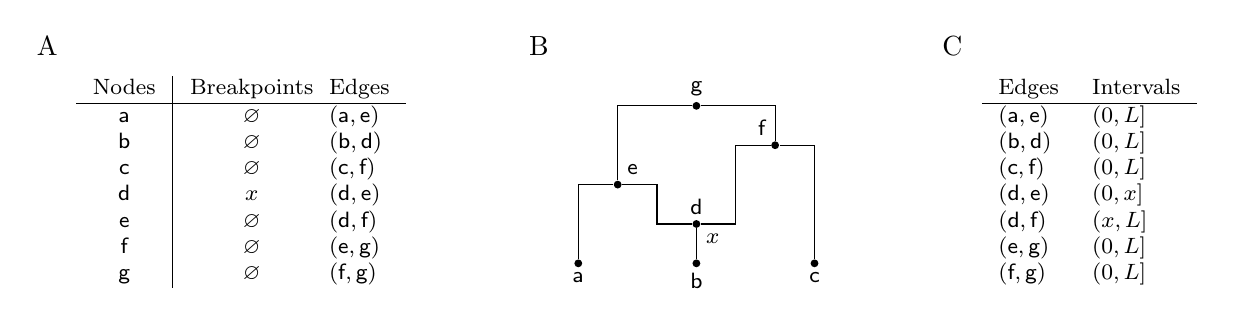
\begin{tikzpicture}[x=5mm, y=5mm, node distance=2mm and 20mm]
\tikzset{greynode/.style={circle,fill,inner sep=1},
nodelabel/.style={font=\footnotesize}}

\node (s0) [greynode] at (0, 0) {};
\node (s1) [greynode] at (3, 0) {};
\node (s2) [greynode] at (6, 0) {};
\node (s3) [greynode] at (3, 1) {};
\node (s4) [greynode] at (1, 2) {};
\node (s5) [greynode] at (5, 3) {};
\node (s6) [greynode] at (3, 4) {};

\node [anchor=north west] at (-1.5,6) {B};
\node [nodelabel,anchor=north west] at ($(s3) + (0,0)$) {$x$};
\foreach \u/\lab in {s0/$\textsf{a}$, s1/$\textsf{b}$, s2/$\textsf{c}$} \node[nodelabel,anchor=north] at (\u) {\lab};
\foreach \u/\lab in {s4/$\textsf{e}$} \node[nodelabel,anchor=south west] at (\u) {\lab};
\foreach \u/\lab in {s5/$\textsf{f}$} \node[nodelabel,anchor=south east] at (\u) {\lab};
\foreach \u/\lab in {s3/$\textsf{d}$, s6/$\textsf{g}$} \node[nodelabel,anchor=south] at (\u) {\lab};

%% Edges
\draw (s1) -- (s3);
\draw (s0) |- (s4);
\draw (s4) -- (2,2) |- (s3);
\draw (s4) |- (s6);
\draw (s3) -- (4,1) |- (s5);
\draw (s2) |- (s5);
\draw (s5) |- (s6);

\node [anchor=north west] at (-14,6) {A};
\node [nodelabel,anchor=north west] at ($(-13,5)$) {
\begin{tabular}{c|c}
% \multicolumn{2}{c}{Breakpoints}\\
Nodes & Breakpoints\\
\hline
$\textsf{a}$ & $\varnothing$ \\
$\textsf{b}$ & $\varnothing$ \\
$\textsf{c}$ & $\varnothing$ \\
$\textsf{d}$ & $x$ \\
$\textsf{e}$ & $\varnothing$ \\
$\textsf{f}$ & $\varnothing$ \\
$\textsf{g}$ & $\varnothing$ \\
\end{tabular}};

\node [nodelabel,anchor=north west] at ($(-7,5)$) {
\begin{tabular}{l}
Edges\\
\hline
$(\textsf{a}, \textsf{e})$ \\
$(\textsf{b}, \textsf{d})$ \\
$(\textsf{c}, \textsf{f})$ \\
$(\textsf{d}, \textsf{e})$ \\
$(\textsf{d}, \textsf{f})$ \\
$(\textsf{e}, \textsf{g})$ \\
$(\textsf{f}, \textsf{g})$ \\
\end{tabular}};


\node [anchor=north west] at (9,6) {C};
\node [nodelabel,anchor=north west] at ($(10,5)$) {
\begin{tabular}{ll}
Edges & Intervals\\
\hline
$(\textsf{a}, \textsf{e})$ & $(0, L]$ \\
$(\textsf{b}, \textsf{d})$ & $(0, L]$ \\
$(\textsf{c}, \textsf{f})$ & $(0, L]$ \\
$(\textsf{d}, \textsf{e})$ & $(0, x]$ \\
$(\textsf{d}, \textsf{f})$ & $(x, L]$ \\
$(\textsf{e}, \textsf{g})$ & $(0, L]$ \\
$(\textsf{f}, \textsf{g})$ & $(0, L]$ \\
\end{tabular}};


\end{tikzpicture}
\caption{\label{fig-arg-data-structure}
A classical ARG (subfigure B), contrasting node with edge breakpoint annotations.
(A) recombination breakpoint information encoded on \emph{nodes}.
This encoding is limited in the patterns of inheritance that can be
described and requires that edges be ordered to avoid ambiguity.
(C) breakpoint annotations associated with \emph{edges}.
Associating the interval of genome inherited by the child node
from the parent with the corresponding edge allows
any pattern genetic inheritance to be described and does
not require edges to be ordered. In this example, each edge is associated
with a single interval, but more generally, multiple non-overlapping intervals
can be associated with a single edge.
}
\end{figure}

% What do we mean by an eARG, formally?
Formally, we can define the classical eARG as a tuple $(e, \sigma)$, where $e$
is an ordered list of edges defining a directed acyclic graph and
$\sigma: \mathbb{N} \rightarrow \mathbb{N}$
is a function mapping nodes to recombination breakpoints,
such that $\sigma(u) = x$
if $u$ is a recombination event with breakpoint $x$ and
$\sigma(u) = \varnothing$ otherwise. (This formulation is equivalent to stipulating that
a recombination node is of a different ``type'' to other nodes,
with breakpoints only associated with that node type).
Each edge $e_j = (c, p)$ describes an edge between
child node $c$ and parent $p$, where $c, p \in \mathbb{N}$.
For each recombination node $u$ we must
have exactly two edges in $e$ such that $u$ is the child.
Note that this description captures only the
graph topology: if we also wish to know the times of events we need
an additional function $t(u): \mathbb{N} \rightarrow \mathbb{R}$
which defines the time of each node.


% % Not sure if we actually include this, but it's good to work it through
% % to make sure the notation works. Maybe something to stick into
% % an appendix
% The most fundamental operation that we need to perform on an ARG
% data structure is extracting the local tree topology at a particular
% position along the genome. The basic strategy is to traverse
% the graph upwards, building the tree as we visit each node.
% At a recombination node, when we have a choice of two parents,
% we follow the path that corresponds to the position that we
% are building the tree for. More precisely, let $S$ be the set
% of sample nodes (usually the leaves of the graph)
% and $0 \leq x < L$ be a position along the genome, and suppose
% we are building a mapping $p_u$ that defines the parent of node
% $u$ at $x$.
% Let $N$ be a set of
% nodes we are currently constructing the tree at,
% and initialise $N \leftarrow S$.
% Then, while $|N| > 0$, we add branches to the
% tree as follows. Let $u$ be an arbitrary element of $N$ (which
% we remove).
% % This isn't right: we're not handling the case where there's
% % no edges in E where the child is $u$.
% Then, if $\sigma(u) < x$ we let $j$ be the
% smallest value such that $e_{j,1} = u$, and otherwise
% let $j$ be the largest value such that $e_{j,1} = u$.
% Then, set $v \leftarrow e_{j, 2}$,
% $p_u \leftarrow v$
% and $N \leftarrow N \cup \{v\}$.

The ordering of edges is a vital element of the eARG encoding.
This is because there is a fundamental ambiguity involved
in associating recombination breakpoints with \emph{nodes}
rather than edges,
and the only way we can break this symmetry is to assign
some meaning to the order in which the parents are listed
(\cite{griffiths1997ancestral} refer to the ``left'' and ``right''
parents of a recombination event). This is usually described
in terms of the process in which we extract the local trees
along the genome from an eARG.
To recover
the tree at genome coordinate $x$,
we traverse the graph rootwards from the leaves. At a particular
node $u$, if it has one parent we are at a common ancestor
node and we follow that parent. If we are at a
recombination node, $u$ has two parents: if
$x$ is less than the breakpoint $\sigma(u)$ we follow
the edge to the first parent, and otherwise follow the edge
to the second parent.
This ordering requirement, while straightforward
to describe, has some practical drawbacks. For example,
% Surely the meaning is clear from the context here and we don't need
% qualify the meaning of ``ARG''
simulating an ARG in this representation is
complicated by the fact that the
first event to occur may hit the lineage carrying the ancestry
to the right of the breakpoint rather
than the left, and so we cannot emit edges as they are generated.
Such issues can be worked around, of course,
but depending on the ordering of otherwise indistinguishable
objects is generally problematic. In practice, several
methods
explicitly associate information with the outbound edges
of a recombination event
to resolve the problem~\citep{lyngso2005minimum,ignatieva2021kwarg}.

% it's not reasonable to assume that one type of event happens
% at a time any more.
The eARG is also limited in the types of ancestral history that can
be described. This ARG encoding is derived from the coalescent
with recombination, which explicitly assumes that only one type
of event can occur (i.e., common ancestry or recombination) at a
time. This model is derived as an approximation to a Wright-Fisher
model, assuming that the sample size $n$ is much less than the
population size $N$, and that the genome is short enough
that the number of extant lineages remains
much smaller than $N$ at all times. These approximations are
reasonable to make for small datasets, such as
the classic \citet{kreitman1983nucleotide} \emph{Drosophila melanogaster}
ADH gene dataset (comprising 11 genomes over 2.7 kb of sequence with 43 SNPs,
see the ``\nameref{ARG_inference_methods}'' section). However,
they are highly questionable in modern datasets. % absurd really
For example, many
human datasets consist of hundreds of thousands of
genomes~\citep{bycroft2018genome,karczewski2020mutational,tanjo2021practical},
and thus our sample size is often much \emph{larger} than $N_e$
(often assumed to be $10^4$ in humans).
The 1000 bull genomes project~\citep{hayes20191000}
comprises close to 7000 genomes, which are part of multi-generation pedigrees
with millions of animals and extensive SNP array genotype and phenotype data \citep[e.g.][]{Cesarani2022}. For example,
the US dairy cattle database alone comprises more than 6 million animals with SNP array genotypes\footnote{\url{https://queries.uscdcb.com/Genotype/counts.html}},
while the effective population size in modern dairy cattle breeds is less than 100 and decreasing~\citep{MacLeod2013,Makanjuola2020}.
This low effective population size is caused by intense selection and
staggering use of a handful of bulls across the world. The current record
holder is the bull Toystory that has produced 2.4 million doses of semen
for artificial insemination across 13 years\footnote{\url{https://www.dairyherd.com/news/world-renowned-toystory-bull-has-died}}.
An extreme sign of these breeding practices is that there are only two ancestral
Y-chromosome linages present in today's US Holstein dairy breed~\citep{Yue2015}.
Similar datasets are becoming available also in other livestock species.
Notably, \citet{RosFreixedes2022} have combined genome
and SNP array data to infer recombination of genomes for 440,610 pigs within
7 multi-generation pedigrees~\citep{whalen2018,Johnsson2021,Ros-Freixedes2020}.
Effective population size in modern pig breeds is also less than 100 due to
intense selection and directed reproduction \citep{Hall2016,Porcnic2016}.
Complete chromosome-level assemblies are now possible
in humans~\citep{miga2020telomere},
and projects are under way to obtain high-quality assemblies
for all eukaryotic species in Britain and Ireland~\citep{darwin2022sequence}
and ultimately worldwide~\citep{lewin2022earth}.
While the coalescent model can be suprisingly robust to
basic violations of the underlying assumptions~\citep{
wakeley2012gene,bhaskar2014distortion,nelson2020accounting},
it is not acceptable that our ability to \emph{represent}
ancestral relationships should be limited by these assumptions.
In a Wright-Fisher model, coalescence and recombination can
occur at the same time in the same genomes, which is increasingly
captured in the incredibly rich datasets that are available today.

A final limitation of the eARG encoding illustrated in
Fig.~\ref{fig-arg-data-structure}A is the inability to represent
multiple recombinations along a chromosome, gene conversion,
or transmission of multiple chromosomes.
[Sentence saying ``gene conversion is important, actually, cite, cite,
so we should be hoping to infer it some day''. Presumably people
already are in bacterial contexts? Gregor: I recall this paper from
Arabidopsis https://www.pnas.org/doi/10.1073/pnas.1211827110]
To allow us to encode data from these important processes we
must either devise workarounds to the event based encoding
(i.e., model gene conversion as two recombination events) or
generalise the model to more appropriately reflect the realities
of modern datasets.

Fortunately, it is straightforward to generalise the classical Griffiths
eARG encoding to both simplify implementations and to encompass any
possible pattern of genetic inheritance.
The only change that we require is to associate
the details of inheritance intervals with \emph{edges} rather than
as breakpoints associated with recombination events and
edge ordering rules. This is illustrated in Fig~\ref{fig-arg-data-structure}C
where this alternative edge annotation formulation is
shown. By associating the interval $(0, x)$ with edge $(d,e)$
and the interval $(x, L)$ with $(d, f)$ we make the encoding
unambiguous: we can list the edges in any order, and it
will describe the same set of local genealogical trees.
This approach is also more flexible, because any pattern
of inheritance can be described by these intervals. For
example, if a gene conversion event occurred where a segment
between between positions $x$ and $y$ was inherited by
node $d$ from $e$, we would state this by associating
the intervals $\{(0, x], (y, L]\}$ with $(d,e)$ and
$\{(x, y]\}$ with $(d,f)$.
This change is straightforward, involves no loss of information
and (as we see in later sections)
greatly increases both the expressivity and computational
power of ancestral recombination graph data structures.

\section*{Genome ARGs}
% We're not the first to talk about ARGs and pedigrees, and we're
% not doing anything controversial.
The deep connection between ARGs and pedigrees is of course
well known
\citep[e.g.][]{wakeley2012genetics,gusfield2014recombinatorics,
speed2015naturereviewsgenetics}
and recent discussions have illustrated the
relationship~\citep{mathieson2020ancestry,brandt2021evaluation}, % more??
showing how the coalescence and recombination events in an ARG
correspond to particular genomes in the pedigree.
As discussed in the previous section, the definition of an ARG
as a \emph{data structure} in terms of these two events is problematic,
fundamentally limiting the patterns of ancestry that can be described.
Following \cite{mathieson2020ancestry} instead of focussing on events,
we define the ARG data structure in terms of \emph{genomes} and the
patterns of transmission between them.
% Bit of duplication here, but good to make the point about being
% motivated by real existing datasets not some academic desire to
% model complexity that isn't there.
This, coupled with
the explicit association of genome coordinates with edges, allows
us to represent even the bewilderingly complex patterns of relatedness
present in modern datasets.

\begin{figure}
\begin{center}
    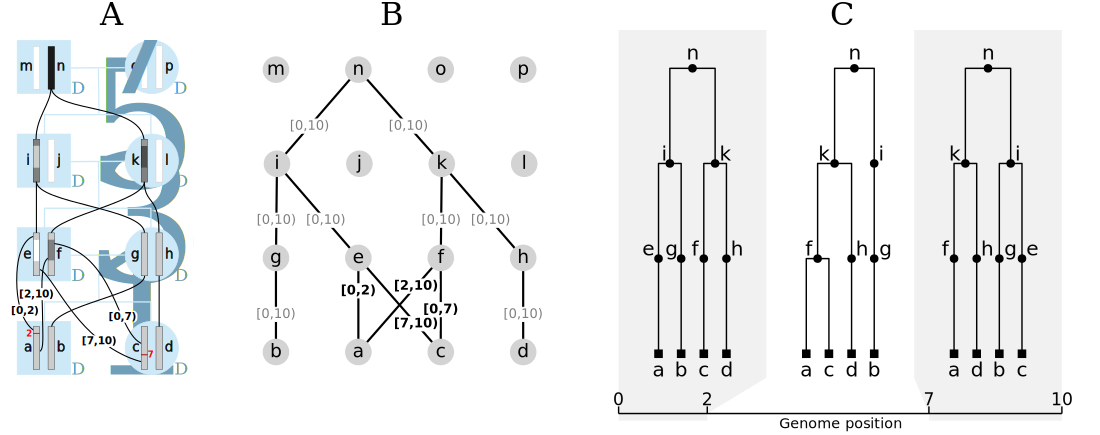
\includegraphics[width=\textwidth]{illustrations/arg-in-pedigree}
\end{center}
\caption{\label{fig-arg-in-pedigree}
% TODO caption needs another pass. One the full section has been written
% it'll be clearer what we need to say in the caption vs the text.
The Ancestral Recombination Graph defined in terms of genomes embedded
in a pedigree. (A) Diploid individuals, visualised in a highly inbred pedigree and
labelled $I_1$ to $I_8$, contain both paternal (left) and maternal (right) genomes
labelled \textsf{a} to \textsf{p}. Black lines show transmission paths connecting
genomes in the current generation (\textsf{a} to \textsf{d}) with their ancestors.
Two recombination breakpoints, at positions 2 and 7 mean that genomes \textsf{a}
and \textsf{c} are independent recombinants of the paternal genomes \textsf{e}
% Gregor: there is some overlap between a and c still (the middle region inherited
% from f) so, a and c are not fully independent!
and \textsf{f}: in these cases the edge annotations have been shown, indicating the
region of genome transmitted. Genomes are shaded such that where, backwards in time,
they merge into a common ancestor, the merged region is darker; this shows that all
genomic regions fully coalesce in genome \textsf{n} in the oldest generation.
(B) The equivalent genome ARG, where there is a single type of node (representing
a genome) along with annotations on all edges; annotations showing partial
transmission are highlighted in bold. Recombination, such as that causing the
breakpoint at position 7, is associated with two parent genomes (\textsf{e} and
\textsf{f}) and a child genome (the recombinant, \textsf{c}).
(C) The edge-annotated genome ARG in (B) fully defines the
local relationships along the genome, as shown in the local
(``marginal'') trees.
}
\end{figure}

To distinguish from the classical event-based encodings,
we call this encoding of an ARG data
structure a ``Genome ARG'', or gARG.
Fig~\ref{fig-arg-in-pedigree} illustrates the basic elements of a gARG.
Fig.~\ref{fig-arg-in-pedigree}A shows the genomes
embedded in an inbred diploid pedigree, in which individuals occur at
discrete generations and carry two genomes. Each individual (labelled
$I_1$ to $I_8$) therefore has a paternal genome (on the left) and a maternal one
(on the right), although the pedigree is only shown for concreteness, and
there is no inherent limitation on mating system, ploidy, or age structure.
A genome is inherited from one of the individual's parents,
and may be the recombined product of that parent's two genomes.
For example, individual $I_1$ has two genomes \textsf{a} and \textsf{b},
inherited from parents $I_3$ and $I_4$. Genome \textsf{a} is the product of
recombining $I_3$'s two genomes \textsf{e} and \textsf{f} at position 2,
whereas \textsf{b} was inherited directly from $I_4$'s genome \textsf{g} without
recombination. Fig.~\ref{fig-arg-in-pedigree}B shows the resulting gARG,
depicting the ancestry of the sample genomes \textsf{a}--\textsf{d}. The graph
topology along with the genome coordinate annotations on the
edges then uniquely defines the trees at every position
along the genome (Fig.~\ref{fig-arg-in-pedigree}C).

Formally, we can define a gARG as a set of edges $E$, where each
element of the set is a tuple $(c, p, I)$ such that $c, p \in \mathbb{N}$,
$c$ is the child node, $p$ is the parent node and $I$ is the set of
disjoint genomic intervals $(\ell, r]$ over which genome $c$ inherits from $p$ (we may
also phrase this in terms of the ancestral material of a sample---see
the next section). Deriving the local tree at a point $x$
follows largely the same pattern as for an eARG but is somewhat
simpler because coordinate information is directly associated with
edges. Starting with the sample nodes $S$ we traverse
rootwards through the graph from child to parent. At each node $u$, we find an
edge $(c, p, I) \in E$ such that $u = c$ and $x \in I$
and move to the next node $p$.

The focus on genomes rather than events has some interesting
and important ramifications. Firstly, a gARG may contain nodes that
do not correspond to any particular event in the ancestry of the samples.
For example, node \textsf{h} is the direct ancestor of \textsf{d} in
Fig~\ref{fig-arg-in-pedigree}, and is not the product of either a
coalescence or a recombination. Such nodes would usually be removed
from the graph so that \textsf{d} descends directly from \textsf{k} (see
the ``\nameref{ARG_simplification}'' section) but there is no necessity for this from
a representational perspective. This ability can be useful in practice and could be
% Do we need to spell this out? Gregor: I think so - see below
required if, for example, we have a deeply sequenced pedigree as in \cite{RosFreixedes2022}.
% e.g. Honeybees? Be great to cite an example!
% Note by Yan - if we actually have the sequence, then this turns into
% a sample node, so would be normally included anyway. Perhaps, therefore
% we should talk about these "pass though" nodes in the context
% of internal samples.
% Gregor: There are no good deeply sequenced pedigrees in honeybees, but sex
% chromosome behaves like haplodiploid system, also any deep pedigree works here, so I cited our pig
% work. Also, I think its important to not think of all genomes as current samples - we have many
% generations of animals with genome or SNP array data and we know pedigree so we can't assume they
% are all current samples - I believe you made this clear distinction also in the tsdate paper with
% ancient human samples

Secondly, unlike in an eARG, nodes in a gARG are not classified into different
types. Indeed a single node can have both multiple children
and multiple parents. This would be the case in Fig~\ref{fig-arg-in-pedigree} if,
for instance, node \textsf{a} were to have two children.
% It is a shame that this is not actually shown in fig 3, but I don't think
% we can do this unless we have 5 generations
Moreover, a single node can have more than 2 children, and (as we shall see in
the ``\nameref{ARG_simplification}'' section), more than 2 parents. Another way to
state this is that transitions between nodes in a gARG can encapsulate multiple
events in an eARG.

The final point deals with the way in which recombination is represented, and is
closely linked to which genomes are chosen as the nodes in a gARG.
We could potentially choose genomes at any point in the life cycle: for instance,
we could chose to represent gametes as ARG nodes. However, the most intuitive
choice is where genomes represent diploid individuals in each generation, as in
Fig~\ref{fig-arg-in-pedigree}A. In this case recombination
is not represented by a single ``recombination node'' (as in an eARG), but with
two parent genomes between which recombination takes place (e.g.
nodes \textsf{e} and \textsf{f}), and a
single resulting ``recombinant'' genome (e.g. \textsf{c}). The
edges that link this recombinant with its two parents carry the information
concerning breakpoint location that would normally be present on the
recombination node in an eARG. For example, node \textsf{c} in
Fig~\ref{fig-arg-in-pedigree} inherits genome positions 0 to 7 from \textsf{f}
and positions 7 to 10 from \textsf{e}, indicating that the breakpoint is at position 7.

% This method for representing recombinations may seem wasteful,
% since more than one node is required for each recombination,
% and genomic interval information must be stored on every edge.
% However, asymptotically the amount of information stored is the
% same, and there is much simplicity to be gained by having
% a single type of node and by treating all edges in the same way.
% More importantly --- as we see in the next section --- we gain the
% ability to simplify the ARG by removing nodes without affecting the
% local tree topologies, and also the ability to record only the
% regions of genome relevant to the final, sample genomes. This last
% feature turns out to be the key to efficient processing of the ARG.

% [Possibly more stuff here: clarify why we assign coordinates to edges
% rather than nodes. Basically lay out all the stuff that we can
% talk about \emph{without} going in to the details of
% ancestry resolution.]


\section*{Ancestry resolution}\label{Ancestry_resolution}
% This is a rough first pass. Will clarify terminology later.
% Need to introduce Hudson's algorithm as concerned with simulating the process of
% the coalescent with recombination as efficiently as possible, and properly merge in
% with this section.

The definition of an ARG as a data structure in terms of
individuals' monoploid genomes
and their direct patterns of inheritance allows us to describe arbitrarily
complex relatedness structures, free from the limitations imposed by
coalescent approximations.
An ARG is an intrinsically retrospective
structure, defined with respect to the ancestry of
a set of sampled genomes.
The graph structure (the nodes and their connectivity through edges)
captures a great deal of information about this ancestry,
but on its own it cannot tell us about the precise relationships between
the samples along the genome: do to this, we must construct the
local (``marginal'') trees.

We can define a sample-resolved gARG as a tuple $(S, E)$
where $S \subset \mathbb{N}$ is a set of sample nodes and
$E$ is a set of edges. Each element of $E$
is a tuple $(c, p, I)$ such that $c, p \in \mathbb{N}$,
$c$ is the child node, $p$ is the parent node and $I$ is the set of
disjoint genomic intervals $(\ell, r]$
over which genome $c$ inherits from $p$, and there is a path from
$c$ to some non-empty subset of $S$ through the local trees.
% Should probably define how we build the local trees somewhere.


\begin{figure}
\centering
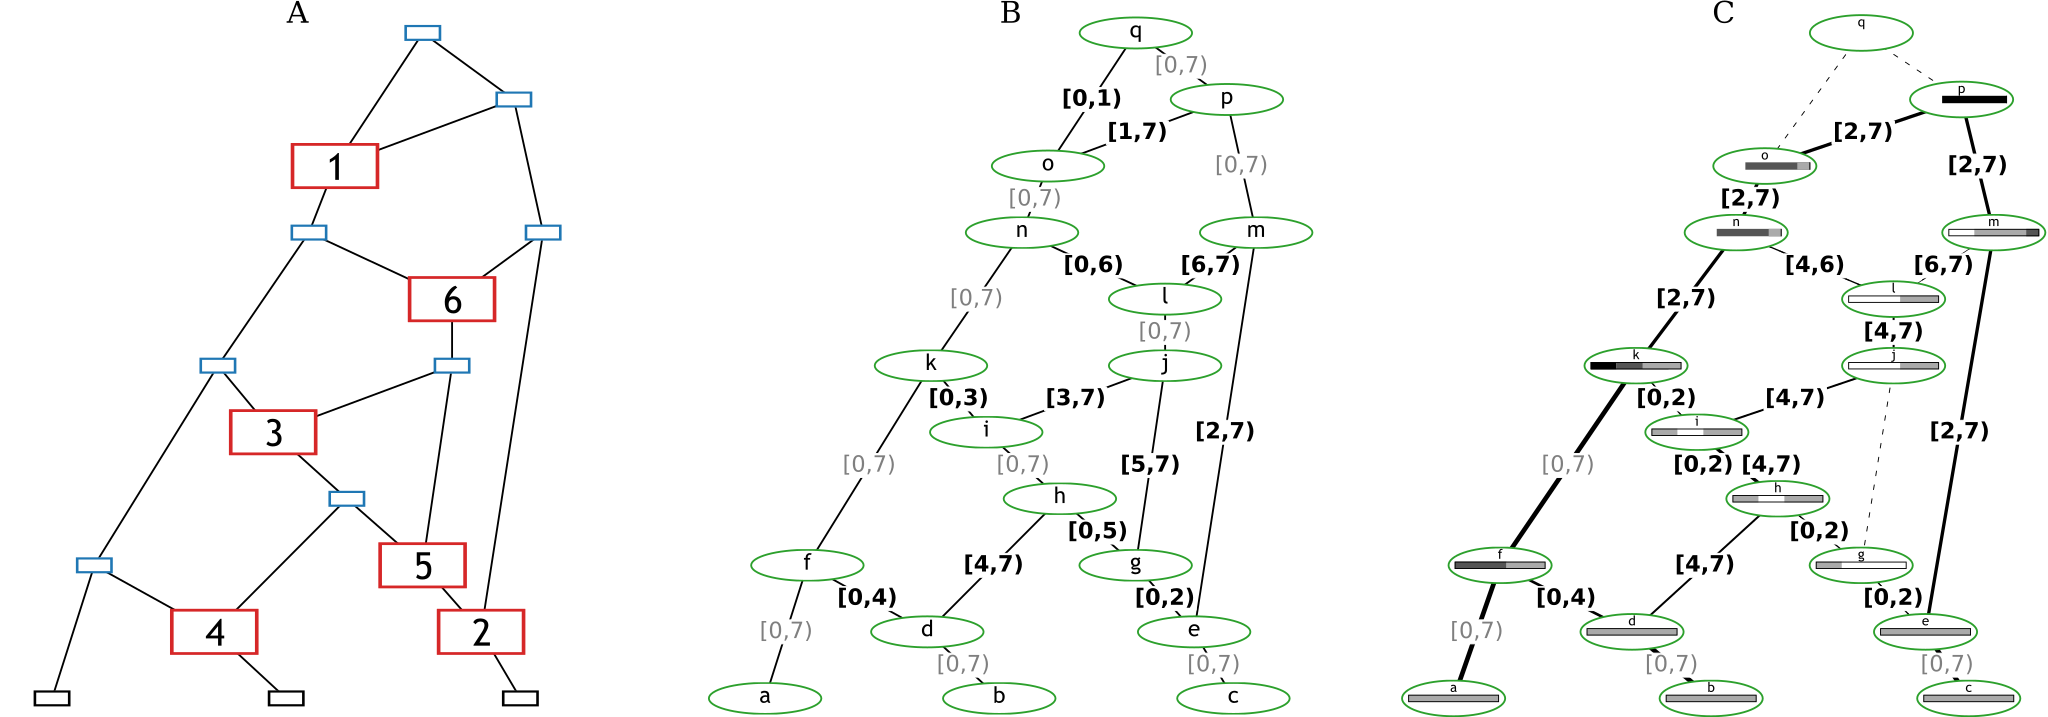
\includegraphics[width=\textwidth]{illustrations/ancestry-resolution}
\caption{\label{fig-ancestry-resolution}
The \citet[][fig. 1]{wiuf1999recombination} example graph as a gARG, with contrasting
edge annotation schemes.
(A) Edge annotations that reflect immediate inheritance, i.e. transmission of
genetic material between parent and child. All edges span the full genome from position 0 to 7,
apart from those linking a recombinant and its two parents (bold).
(B) Sample-resolved edge annotations: the Hudson simplification algorithm has been used to
shorten edge spans to reflect only the upwards transmission of genetic
material from the samples \textsf{a}, \textsf{b}, and \textsf{c}. The depiction of the genome within
each node is shaded as in figure \ref{fig-arg-in-pedigree}a to show
coalescing regions of genome back to the grand MRCA genome \textsf{w}.
In this case, using line widths to reflect the genomic span of each edge can
help to visualise the relative importance of different transmission pathways.
}
\end{figure}

% We should talk about ARG and HUD here. Fig~\ref{fig-ancestry-resolution}A shows
% ARG (the Griffiths graph). However, we have a small issue that subfig B
% doesn't strictly show HUD, because it doesn't terminate as soon as all samples have coalesced.
% We could potentially colour the top (non-HUD) section of the plot in a different colour?

Given a gARG $E$ and the set of samples $S$ we can \emph{resolve} its
ancestry by noting that the resolved interval $Ir$ on an edge $(c,p,I)$
is given by [Rough notes]

\begin{itemize}
\item The ``ancestry interval'' $A_u$ of a node $u$ is the union of
all $R_{u, v}$ for all the children $v$ of $u$. (this isn't quite right)
\item The resolved interval is then the intersection of $A_u$ and the
original inheritance interval $I_v$ on the edge.
\item It would be good of if differentiate between the inheritance intervals
 from the gARG and the ancestry intervals of the resolved gARG.
\end{itemize}

This process is illustrated in Fig~\ref{fig-ancestry-resolution}. It is intimately linked to
Hudson's algorithm which operates by
tracking segments of ancestral material carried by ancestors as
we go backwards in time.

% jk-note unclear here about the best choice of notation. We could have
% lists of tuples (l, r, a), or a tuple of vectors (l_j, r_j, a_j),
% of a tuple (I_j, a_j), where I is a vector of intervals. Going to
% stick with the original tuple notation for now.
%
% Each lineage consists of a set of
% equal-length vectors $\mathbf{l}$, $\mathbf{r}$ and $\mathbf{a}$
% such that for each $1 \leq j \leq \left| l \right|$,
% $[\mathbf{l}_j, \mathbf{r}_j)$ is a half-closed genomic interval and
% $\mathbf{a}_j$ is an integer
% tracking the number of samples the lineage is ancestral to over the interval.
% Assume that the intervals are sorted from left-to-right so that $\mathbf{l}_1$
% and $\mathbf{r}_{|\mathbf{r}|}$ are the left- and right-most positions
% covered by the lineage, respectively.
Each lineage consists of a list of
disjoint ancestry segments $(\ell, r, a)$, where
$[\ell, r)$ is a half-closed genomic interval and $a$ is an integer
tracking the number of samples to which the lineage is ancestral over that interval.
(We also usually track the tree node associated with each segment, but
that is not important for our purposes here so we omit it.)
If we have $n$ samples and a genome of length $m$, the process begins with $n$ lineages
of the form $\{(0, m, 1)\}$. The process then works backwards in time from
the present day as a series of random common ancestor or recombination events.
Recombination events occur at a rate determined by the amount of ancestral material and
the way in which it is distributed along a chromosome.
Let $L$ be the set of ancestors at a given time $t$. Recombination events
happen at rate $\rho \nu / (m - 1)$ where
\[
\nu = \sum_{x \in L}\left( \max_{(\ell, r, a) \in x}r
    - \min_{(\ell, r, a) \in x}\ell - 1 \right)
\]
is the number of available `links' that may be broken. Thus, the rate of
recombination is determined by the left- and right-most extent of the
ancestral material carried by each lineage. At a recombination
event we choose one of these links uniformly and break it. Given a lineage
$x = [(\ell_j, r_j, a_j)]$ and a breakpoint $k$, we have two lineages
$x_1$ and $x_2$ such that FILL IN DETAILS

When $k = |L|$ lineages are present, common ancestor events
occur at rate $\binom{k}{2}$. In a common ancestor event, two lineages
are chosen uniformly at random and their ancestry segments merged.
If we have overlapping intervals of ancestry from the two lineages,
say, $(\ell, r, a_1)$ and $(\ell, r, a_2)$, a
\emph{coalescence} occurs and ancestor represented by the current event
will be present as a node (at least) in the marginal trees covering
the interval $[\ell, r)$. The result of this coalescence is a segment
$(\ell, r, a_1 + a_2)$, and if $a_1 + a_2 < n$ it is included in the
ancestry for the new lineage. Otherwise, if $a_1 + a_2 = n$ we know that
we have found the most recent common ancestor of all samples in
the interval $[\ell, r)$ and so we do not need to simulate its history any further.
Nonoverlapping intervals of ancestry from the two lineages are included
in the resulting lineage without changes. Eventually, as the process continues,
we find resultant lineages in which all segments have fully coalescenced,
and so the number of extant lineages gradually dwindles down to zero.

% Potentially useful text from a previous iteration:
% Wiuf and Hein's classical pair of papers
% clarified the relationship between Hudson's algorithm and the ARG.
% ARG simulation is inherently less efficient than Hudson's
% algorithm because we must track all lineages, even those that correspond
% to sections that have coalesced, or we won't have a complete ARG.

The state-space of the Griffiths process is much simpler than Hudson's algorithm,
which greatly facilitates mathematical reasoning. This simplicity comes at a
substantial cost, however, if we wish to use it as a practical means of
simulating recombinant ancestry. The big ARG is vast, and any realisation
for even moderate levels of recombination is far too large to be of practical
use. The number of events in the big ARG all the way back to the GMRCA
is $O(e^\rho)$~\citep{griffiths1997ancestral}, whereas the number
of events required to simulate the little ARG is
$O(\rho^2)$~\citep{hein2004gene,baumdicker2021efficient}.
This disparity in the number of events in the two formulations is
because the majority of the events that occur in the big ARG do
not affect the genetic ancestry of the sample in any way. Recombination
events that occur outside of ancestral material do not have any bearing
on the ancestry of the sample, and so the structure is hugely redundant.
As~\cite{wiuf1999recombination} note,
``an `ancestral' sequence in the birth and death process
need not have any genetic material in common with a
sequence descended from it.''
% Full quote:
% This process simplifies mathematics on the account that the notion of an
% ancestor will have a less restrictive meaning than usual:
% An ``ancestral'' sequence in the birth and death process
% need not have any genetic material in common with a
% sequence descended from it.


\section*{ARG simplification}\label{ARG_simplification}

Not all nodes in an ARG are equal. Assuming that we have sequenced the
genomes of the samples, there are intrinsic limits on what can
be known about more ancient nodes, determined by the graph topology
and the flow of ancestral material through it.
\emph{Simplification}~\citep{kelleher2018efficient} is the process
of removing nodes and re-writing edges in a gARG to remove
various types of redundancy, while maintaining the crucial properties
that the ``meaningful'' topology in the local trees is not affected,
and the relationship between nodes in adjacent trees is maintained.

\begin{figure}
\centering
\vspace{5em}
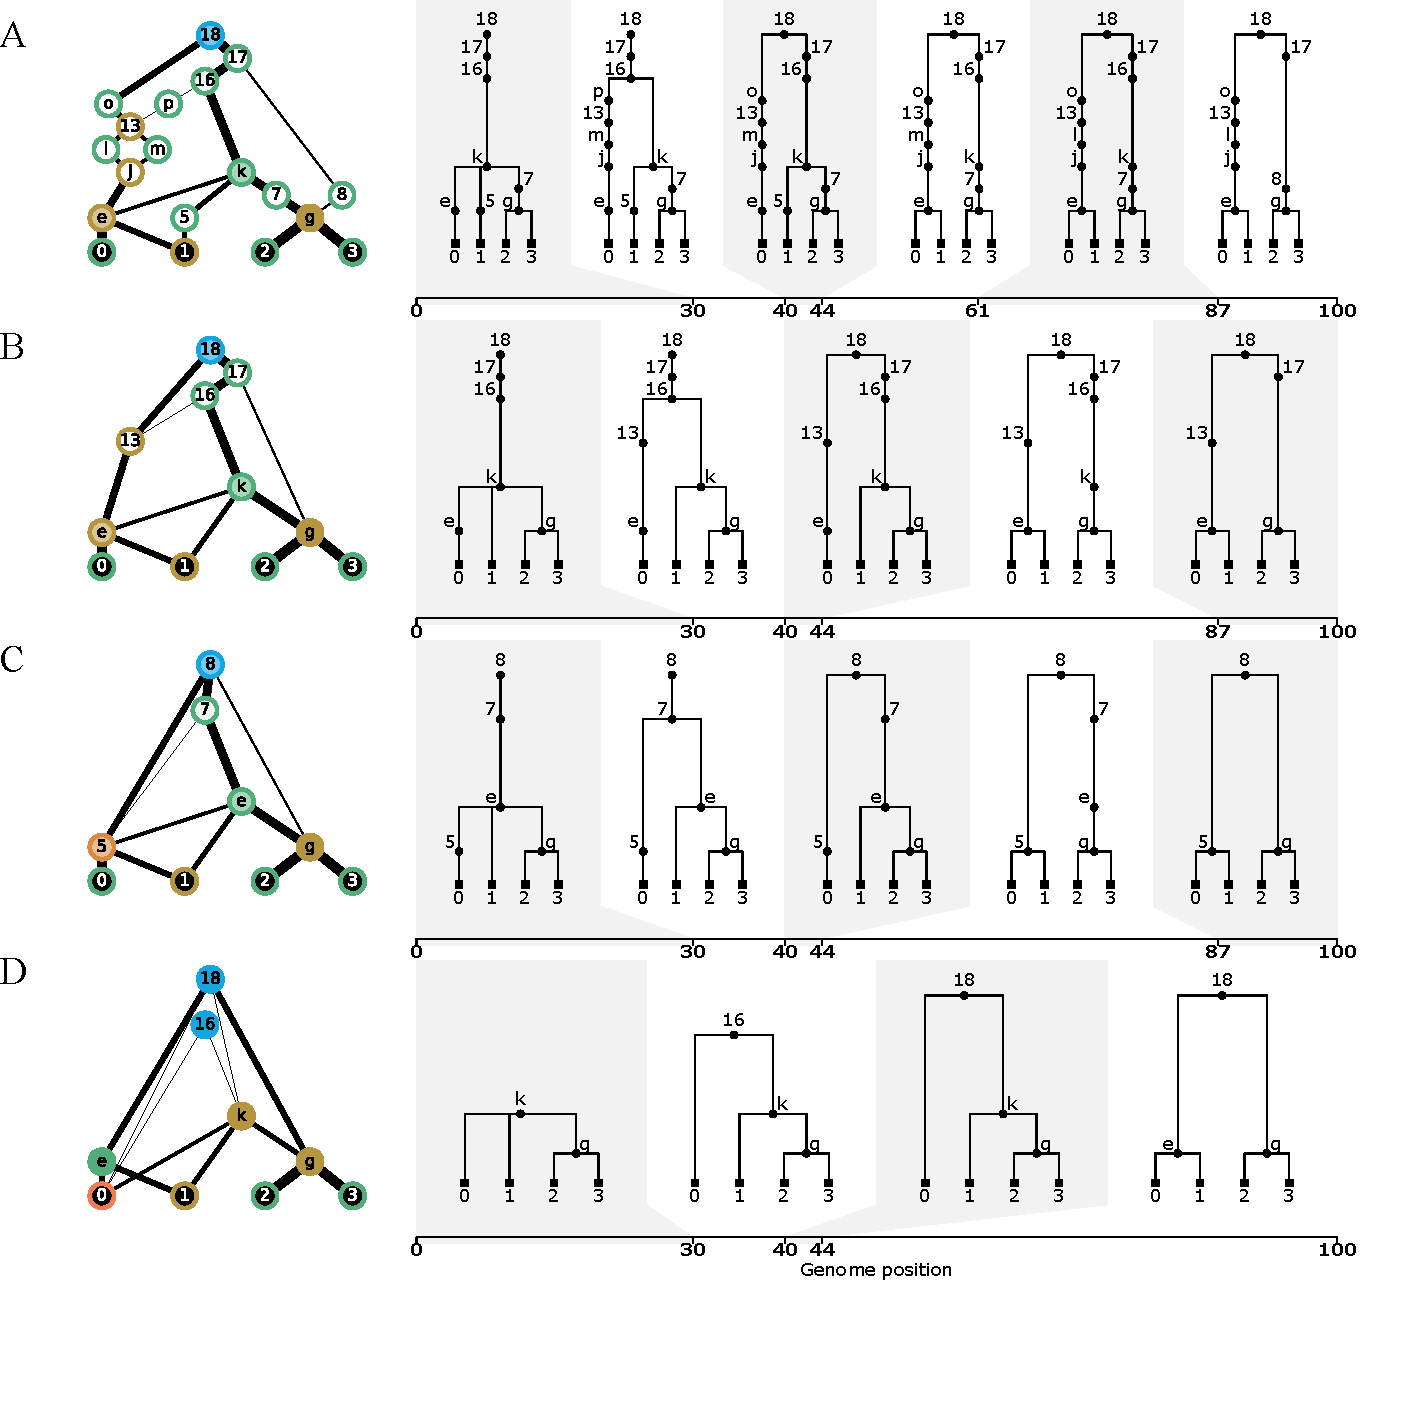
\includegraphics[width=\linewidth]{illustrations/simplification}
\caption{\label{fig-simplification}
ARG simplification. In all cases the graph visualization is shown on the left
and the equivalent marginal trees on the right.
(A) A gARG simulated from a diploid Wright-Fisher
model. Note that the genome \textsf{k} has three children, and the genomes
\textsf{e} and \textsf{g} simultaneously have multiple parents and multiple children;
neither could be directly represented in a Griffiths-like eARG encoding
(see the ``\nameref{eARG}'' section). The penultimate local tree is highlighted to aid discussion.
(B) Simplified to remove all
% trying out this terminology - can define in the text
1-connected graph components (e.g., diamonds such as \textsf{jlnm}).
(C) Remove nodes that are unary in all local trees. This removes both recombinant nodes
that have only one child (e.g. \textsf{n}) and nodes that have more
than one child (i.e. are ``common ancestors'') but never represent coalescences
in the local trees (e.g. \textsf{r}).
(D) Rewrite edges to bypass any unary nodes in local trees. Note that this loses lineage
information such as the fact that \textsf{k} is connected to \textsf{a} via \textsf{e}.
}
\end{figure}

% Q: would it help to talk about ``tree vertices'' here or would it
% just be more confusing? I worry that people would think that
% they are two different things then, and it's really important
% that they get that a node-is-a-node


The ideas of ``meaningful'' local tree topologies revolve around the
presence of ``unary'' nodes: a node in the tree that has exactly
one child. Fig.~\ref{fig-simplification} show a series of successive steps of
simplification, starting with a complete gARG simulated under a Wright-Fisher
model, shown both as a graph on the left, and the equivalent set of 6
local trees on the right (Fig.~\ref{fig-simplification}A). Consider the path above node
\textsf{a} in the penultimate tree, highlighted in yellow and covering genomic positions
60 to 70. On this path, before \textsf{a} meets its common ancestor with the other samples at
node \textsf{q}, it passes through  \textsf{e},  \textsf{j},  \textsf{m},  \textsf{n} and
\textsf{p}, which in this region of the genome are all unary nodes. This reflects the
passage of this span of genome through the ARG towards the root (see the
``\nameref{Ancestry_resolution}'' section).
Such unary nodes in a local tree are not usually considered important,
because they provide very little information and are not
detectable by information from the tree. % weak
The nodes in a tree usually mark the points where samples find a
 \emph{common} ancestor, such as node \textsf{q} in the highlighted
tree. For many purposes, we would therefore consider a path directly
joining sample \textsf{a} to node \textsf{q} to be of equivalent status to the path
containing the intermediate unary nodes. Simplification is the process of removing
these less informative and (for most computational purposes) inefficient nodes
from the local trees and the corresponding annotated graph.

The first type of simplification that we can perform is to remove
graph topology that is invisible to the samples. The most well
known example of such topology is a so-called
``diamond''~\citep{rasmussen2014genome}
in which the two parent nodes of a recombination immediately
join again into a common ancestor (e.g. \textsf{j}, \textsf{l}, \textsf{m}
and  \textsf{n} in Fig.~\ref{fig-simplification}A).
Unless we are specifically
interested in the recombination event or ancestral genomes,
there is no information in this topology and the diamond can be
replaced by a single edge. More generally, any
subgraph which is singly-connected in both the leafward and
rootward direction (a ``super-diamond'') is non-identifiable and can be
replaced by a single edge. This definition includes the case
of a single node that has one inbound and one outbound edge, such as
nodes \textsf{f} and \textsf{h}.
Fig.~\ref{fig-simplification}B shows the result of this type of
graph topology simplification.

Simplifying away diamonds will remove many unary nodes from the
local trees, but there can still be nodes that are unary in all
of the local trees. In particular, a node can represent a recombinant
with multiple parents in the graph but only a single child (e.g. node \textsf{n}
in Fig.~\ref{fig-simplification}B), or can represent a common ancestor with
multiple children in the graph but in which no local coalescence takes place
(node \textsf{r} in Fig.~\ref{fig-simplification}B).
% point out that this is why Hudson refers to CA nodes, not coalescence nodes
Such nodes are not singly connected in the graph, but are nevertheless unary in
all of the local trees in Fig.~\ref{fig-simplification}B. The operation to remove them,
the results of which are shown in Fig.~\ref{fig-simplification}C,
therefore requires knowledge not just of the graph topology, but also of the
edge annotations. Removal of recombinant nodes can produce graph nodes with
more than 2 parents (e.g. node \textsf{e}); likewise, removal of
common ancestor but non-coalescent nodes can produce graph nodes with
more than 2 children (e.g. node \textsf{s}). These represent a ``stacking up'' of multiple
often indistinguishable events into a single node, something which is impossible
to encode in an eARG.

The remaining nodes are MRCAs of some subset of the samples
at \emph{some} positions along the genome. We still have
some unary nodes in the local trees, but these nodes will
correspond to a coalescence in at least one other
local tree. For example, node  \textsf{k} is unary in the second tree
of Fig.~\ref{fig-simplification}C, but is either binary
or ternary in all subsequent trees (recall this is a Wright-Fisher
simulation). The final level of simplification is to alter the edge annotations
such that, although no nodes are removed from the graph, \emph{all}
unary nodes disappear from the local trees (Fig.~\ref{fig-simplification}D).
It is common for this operation to remove nodes above the top MRCA node
in the tree, resulting in many more root nodes (here, \textsf{q} and \textsf{k}
become roots). [And continue]
% Note that although this last stage produces much simpler local trees, by
% removing information about the exact paths taken by lineages through
% the graph, it loses potentially important information about shared edges
% between trees. It is not clear whether (c) or (d) leads to a more compact
% representation of the ARG in terms of number of edges.

\section*{ARGs and SPRs}
\citet{wiuf1999ancestry,wiuf1999recombination} recast
the coalescent with recombination
as a stochastic process along the genome rather than backwards in time.
In this formulation we begin at one end of a chromosome by
sampling a tree under the standard coalescent, and then reason
about how this tree is modified by recombination events
as we move along the genome. Although this algorithm is
significantly more complicated to simulate than Hudson's
backwards in time approach, it has led to substantial
insights into the process of recombination itself
and to the sequentially Markov Coalescent (SMC)
approximations~\citep{mcvean2005approximating,marjoram2006fast}
that are central to many modern methods.

Under the coalescent with recombination (or SMC) each local
tree along the genome is transformed into the next by
a ``subtree prune-and-regraft'' (SPR)
% Hein et al call it the "subtree transfer" operation but it's
% the same thing.
operation~\citep{hein1990reconstructing,song2003on,song2006properties}.
The number of SPRs required to transform one leaf-labelled tree
into another is known as the SPR distance
% Hein 1996 say that SPR distance is NP-hard, but Allen 2001
% say this is wrong. But then Bordewich went ahead and said
% yes, actually it is NP hard.
and is NP-hard to
compute~\citep{hein1996complexity,allen2001subtree,bordewich2005computational}.

[Discussion of SPRs in an EARG]

The effects of recombination as we move from left-to-right along
the genome in an unsimplified gARG are easy to interpret.
Consider the highlighed tree in Fig~\ref{fig-simplification}A.
In it the parent of \textsf{e} is \textsf{j}, whereas in the next tree
its parent is \textsf{k}. Since both parents are present as
unary nodes in the tree, we simply change one edge in
order to effect the transition.
% Need revising to fit new example
A more complex transition occurs when we have a regraft operation
that occurs above the current root (i.e., the current oldest
non-unary node). For example, the transition between the
second and third trees corresponds to node D switching
from the path through I to H, and we then must add branches
corresponding to passing through L and meeting at M.

The equivalence between an ARG and a set of local trees
separated by SPRs is often mentioned [e.g. x y z], but
it is important to note that while extracting local
trees from an ARG is straightforward, the converse
process of reconstructing precisely the same ARG from
these trees is more problematic. If the internal
nodes are consistently labelled and unary nodes are
included in the local trees (e.g., Fig~\ref{fig-simplification})
then it is easy to exactly reconstruct the ARG.
Otherwise, the problem is much more difficult and it
may not be possible to uniquely reconstruct the original ARG.
Without labels for the internal nodes, we are forced to
to reason about which subtrees remain the same and which
differ due to the SPR separating adjacent trees in order to
assign node identity. Without the internal unary nodes marking
recombinations, we must infer their existence. In
general, there will not be a unique solution to this problem,
and so there can be many possible ARGs compatible with
a given list of
% want to say "standard phylogenetic" trees here or something, but
% and they don't have to be binary (just arity > 1), but thought
% this would be familiar to readers?
% Jere: Could just say leaf-labelled "marginal trees", "ancestral trees",
% "local trees", or something like that.
leaf-labelled binary trees.

[ Cite \citep{deng2021distribution} somewhere here.]

% This text might go somewhere
% We may have nodes corresponding to genomes that are ancestral to
% the sample along their entire span
% (e.g.\ node $H$ in Fig.~\ref{fig-ancestry-resolution}),
% genomes that carry no genetic material ancestral to the sample at all
% (e.g.\ node $J$ in Fig.~\ref{fig-ancestry-resolution}),
% and every possibility along the continuum between these extremes.
% Clearly, we can only ever hope to infer the fraction of an ancestor's
% genome that is ancestral to the sample.

\begin{figure}[ht]
\centering
% FIXME this is a quick nasty hack to make the figure a bit smaller and
% prevent flushing all the other figures to the end of the document.
\scalebox{0.5}{
\begin{tabular}{cc}
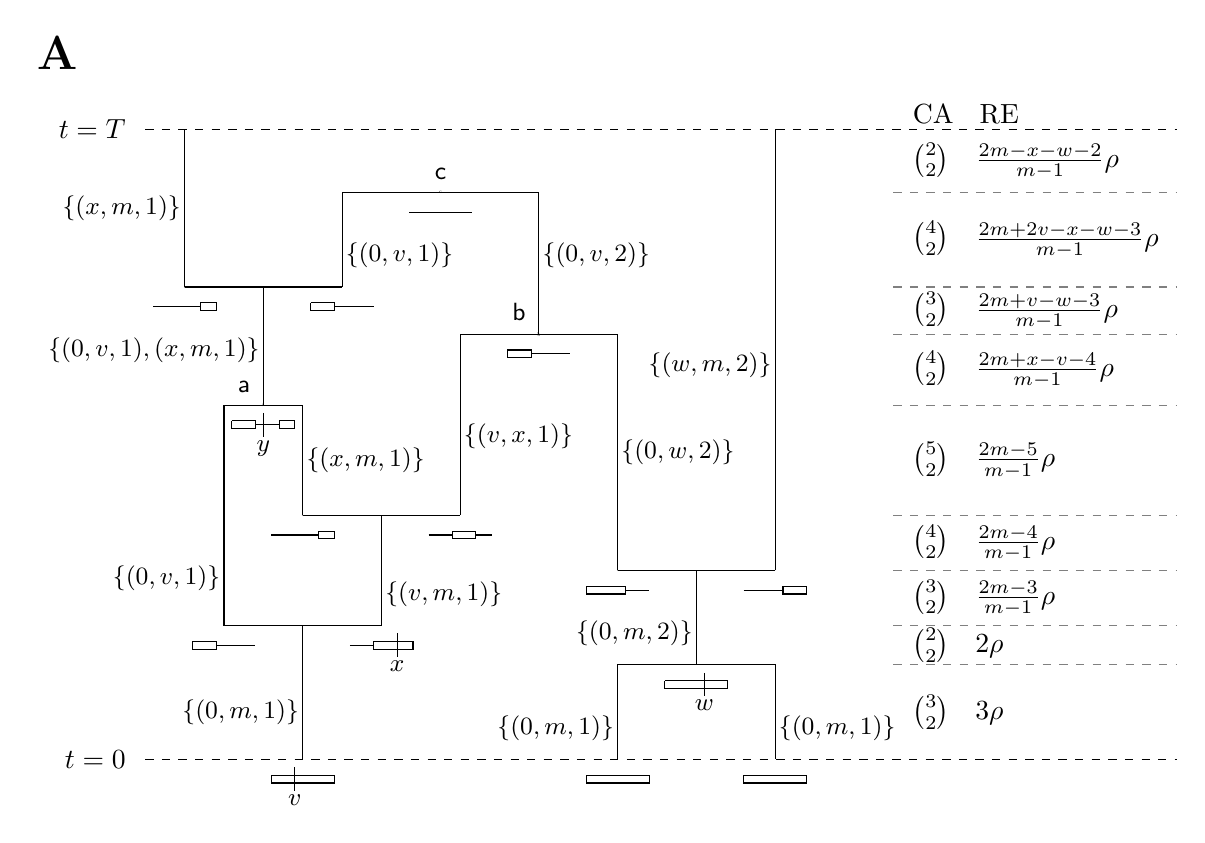
\begin{tikzpicture}
	\node [anchor=north west] at (-3.5,9.3) {\LARGE \textbf{A}};
	\draw (-0.4, -0.2) -- (0.4, -0.2) -- (0.4, -0.3) -- (-0.4, -0.3) -- (-0.4, -0.2);
	\draw (-0.1, -0.1) -- (-0.1, -0.4);
	\node [label=below:{\small $v$}] at (-0.1, -0.2) {};
	\draw (3.6, -0.2) -- (4.4, -0.2) -- (4.4, -0.3) -- (3.6, -0.3) -- (3.6, -0.2);
	\draw (5.6, -0.2) -- (6.4, -0.2) -- (6.4, -0.3) -- (5.6, -0.3) -- (5.6, -0.2);

	\draw (4,0) -- (4, 1.2) -- (6, 1.2) -- (6,0);
	\draw (4.6, 1) -- (5.4, 1) -- (5.4, 0.9) -- (4.6, 0.9) -- (4.6, 1);
	\draw (5.1, 1.1) -- (5.1, 0.8);
	\node [label=below:{\small $w$}] at (5.1, 1) {};

	\draw (0, 0) -- (0, 1.7) -- (-1,1.7) -- (1,1.7);
	\draw (-1.4, 1.5) -- (-1.1, 1.5) -- (-1.1, 1.4) -- (-1.4, 1.4) -- (-1.4, 1.5);
	\draw (-1.1, 1.45) -- (-0.6, 1.45);
	\draw (0.6, 1.45) -- (0.9, 1.45);
	\draw (0.9, 1.5) -- (1.4, 1.5) -- (1.4, 1.4) -- (0.9, 1.4) -- (0.9, 1.5);
	\draw (1.2, 1.6) -- (1.2, 1.3);
	\node [label=below:{\small $x$}] at (1.2, 1.5) {};

	\draw (5, 1.2) -- (5, 2.4) -- (4,2.4) -- (6,2.4);
	\draw (3.6, 2.2) -- (4.1, 2.2) -- (4.1, 2.1) -- (3.6, 2.1) -- (3.6, 2.2);
	\draw (4.1, 2.15) -- (4.4, 2.15);
	\draw (5.6, 2.15) -- (6.1, 2.15);
	\draw (6.1, 2.2) -- (6.4, 2.2) -- (6.4, 2.1) -- (6.1, 2.1) -- (6.1, 2.2);

	\draw (1, 1.7) -- (1, 3.1) -- (0,3.1) -- (2,3.1);
	\draw (-0.4, 2.85) -- (0.2, 2.85);
	\draw (0.2, 2.9) -- (0.4, 2.9) -- (0.4, 2.8) -- (0.2, 2.8) -- (0.2, 2.9);
	\draw (1.6, 2.85) -- (1.9, 2.85);
	\draw (1.9, 2.9) -- (2.2, 2.9) -- (2.2, 2.8) -- (1.9, 2.8) -- (1.9, 2.9);
	\draw (2.2, 2.85) -- (2.4, 2.85);

	\draw (-1, 1.7) -- (-1, 4.5) -- (0,4.5) -- (0,3.1);
	\node [scale=0.2,label=above left:{\small \textsf{a}}] at (-0.5,4.5) {a};
	\draw (-0.9, 4.3) -- (-0.6, 4.3) -- (-0.6, 4.2) -- (-0.9, 4.2) -- (-0.9, 4.3);
	\draw (-0.6, 4.25) -- (-0.3, 4.25);
	\draw (-0.3, 4.3) -- (-0.1, 4.3) -- (-0.1, 4.2) -- (-0.3, 4.2) -- (-0.3, 4.3);
	\draw (-0.5, 4.4) -- (-0.5, 4.1);
	\node [label=below:{\small $y$}] at (-0.5, 4.3) {};

	\draw (4,2.4) -- (4,5.4) -- (2,5.4) -- (2,3.1);
	\node [scale=0.2,label=above left:{\small \textsf{b}}] at (3,5.4) {b};
	\draw (2.6, 5.2) -- (2.9, 5.2) -- (2.9, 5.1) -- (2.6, 5.1) -- (2.6, 5.2);
	\draw (2.9, 5.15) -- (3.4, 5.15);

	\draw (-0.5, 4.5) -- (-0.5, 6) -- (-1.5,6) -- (0.5,6);
	\draw (-1.9, 5.75) -- (-1.3, 5.75);
	\draw (-1.3, 5.8) -- (-1.1, 5.8) -- (-1.1, 5.7) -- (-1.3, 5.7) -- (-1.3, 5.8);
	\draw (0.1, 5.8) -- (0.4, 5.8) -- (0.4, 5.7) -- (0.1, 5.7) -- (0.1, 5.8);
	\draw (0.4, 5.75) -- (0.9, 5.75);

	\draw (0.5, 6) -- (0.5, 7.2) -- (3,7.2) -- (3,5.4);
	\node [scale=0.2,label=above:{\small \textsf{c}}] at (1.75,7.2) {c};
	\draw (1.35, 6.95) -- (2.15, 6.95);

	\draw (-1.5, 6) -- (-1.5, 8);
	\draw (6, 2.4) -- (6, 8);

	% Edge annotations above each event
	\node [label=left:{\small$\{(0,m,1)\}$}] at (0.2,0.6) {};
	\node [label=left:{\small$\{(0,m,1)\}$}] at (4.2,0.4) {};
	\node [label=right:{\small$\{(0,m,1)\}$}] at (5.8,0.4) {};
	\node [label=left:{\small$\{(0,m,2)\}$}] at (5.2,1.6) {};
	\node [label=left:{\small$\{(0,v,1)\}$}] at (-0.8,2.3) {};
	\node [label=right:{\small$\{(v,m,1)\}$}] at (0.8,2.1) {};
	\node [label=right:{\small$\{(0,w,2)\}$}] at (3.8,3.9) {};
	\node [label=left:{\small$\{(w,m,2)\}$}] at (6.2,5) {};
	\node [label=right:{\small$\{(x,m,1)\}$}] at (-0.2,3.8) {};
	\node [label=right:{\small$\{(v,x,1)\}$}] at (1.8,4.1) {};
	\node [label=left:{\small$\{(0,v,1), (x,m,1)\}$}] at (-0.3,5.2) {};
	\node [label=right:{\small$\{(0,v,2)\}$}] at (2.8,6.4) {};
	\node [label=left:{\small$\{(x,m,1)\}$}] at (-1.3,7) {};
	\node [label=right:{\small$\{(0,v,1)\}$}] at (0.3,6.4) {};

	% Dashed lines for start and end times
	\draw[dashed] (-2, 0) -- (11.1, 0);
	\node [label=left:{$t = 0$}] at (-2,0) {};
	\draw[dashed] (-2, 8) -- (11.1, 8);
	\node [label=left:{$t = T$}] at (-2,8) {};

	% Numbers of extant ancestors and links, from top to bottom
	\node[label=right:{CA \; RE}] at (7.5, 8.2) {};
	\node[label=right:{$\binom{2}{2}$ \; $\frac{2 m - x - w - 2}{m - 1} \rho$}] at (7.5, 7.6) {};
	\node[label=right:{$\binom{4}{2}$ \; $\frac{2 m + 2 v - x - w - 3}{m - 1} \rho$}] at (7.5, 6.6) {};
	\node[label=right:{$\binom{3}{2}$ \; $\frac{2 m + v - w - 3}{m - 1} \rho$}] at (7.5, 5.7) {};
	\node[label=right:{$\binom{4}{2}$ \; $\frac{2 m + x - v - 4}{m - 1} \rho$}] at (7.5, 4.95) {};
	\node[label=right:{$\binom{5}{2}$ \; $\frac{2 m - 5}{m - 1} \rho$}] at (7.5, 3.8) {};
	\node[label=right:{$\binom{4}{2}$ \; $\frac{2 m - 4}{m -1} \rho$}] at (7.5, 2.75) {};
	\node[label=right:{$\binom{3}{2}$ \; $\frac{2 m - 3}{m - 1} \rho$}] at (7.5, 2.05) {};
	\node[label=right:{$\binom{2}{2}$ \; $2 \rho$}] at (7.5, 1.45) {};
	\node[label=right:{$\binom{3}{2}$ \; $3 \rho$}] at (7.5, 0.6) {};

	% Gray dashed lines to visually separate holding times
	\draw[color=gray, dashed] (7.5, 1.2) -- (11.1, 1.2);
	\draw[color=gray, dashed] (7.5, 1.7) -- (11.1, 1.7);
	\draw[color=gray, dashed] (7.5, 2.4) -- (11.1, 2.4);
	\draw[color=gray, dashed] (7.5, 3.1) -- (11.1, 3.1);
	\draw[color=gray, dashed] (7.5, 4.5) -- (11.1, 4.5);
	\draw[color=gray, dashed] (7.5, 5.4) -- (11.1, 5.4);
	\draw[color=gray, dashed] (7.5, 6) -- (11.1, 6);
	\draw[color=gray, dashed] (7.5, 7.2) -- (11.1, 7.2);
\end{tikzpicture}
&
\begin{tikzpicture}
	\node [anchor=north west] at (-3.5,9.3) {\LARGE \textbf{B}};
	\draw (-0.4, -0.2) -- (0.4, -0.2) -- (0.4, -0.3) -- (-0.4, -0.3) -- (-0.4, -0.2);
	\draw (-0.1, -0.1) -- (-0.1, -0.4);
	\node [label=below:{\small $v$}] at (-0.1, -0.2) {};
	\draw (3.6, -0.2) -- (4.4, -0.2) -- (4.4, -0.3) -- (3.6, -0.3) -- (3.6, -0.2);
	\draw (5.6, -0.2) -- (6.4, -0.2) -- (6.4, -0.3) -- (5.6, -0.3) -- (5.6, -0.2);

	\draw (4,0) -- (4, 1.2) -- (6, 1.2) -- (6,0);
	\draw (4.6, 1) -- (5.4, 1) -- (5.4, 0.9) -- (4.6, 0.9) -- (4.6, 1);
	\draw (5.1, 1.1) -- (5.1, 0.8);
	\node [label=below:{\small $w$}] at (5.1, 1) {};

	\draw (0, 0) -- (0, 1.7) -- (-1,1.7) -- (1,1.7);
	\draw (-1.4, 1.5) -- (-1.1, 1.5) -- (-1.1, 1.4) -- (-1.4, 1.4) -- (-1.4, 1.5);
	\draw (-1.1, 1.45) -- (-0.6, 1.45);
	\draw (0.6, 1.45) -- (0.9, 1.45);
	\draw (0.9, 1.5) -- (1.4, 1.5) -- (1.4, 1.4) -- (0.9, 1.4) -- (0.9, 1.5);
	\draw (1.2, 1.6) -- (1.2, 1.3);
	\node [label=below:{\small $x$}] at (1.2, 1.5) {};

	\draw (5, 1.2) -- (5, 2.4) -- (4,2.4) -- (6,2.4);
	\draw (3.6, 2.2) -- (4.1, 2.2) -- (4.1, 2.1) -- (3.6, 2.1) -- (3.6, 2.2);
	\draw (4.1, 2.15) -- (4.4, 2.15);
	\draw (5.6, 2.15) -- (6.1, 2.15);
	\draw (6.1, 2.2) -- (6.4, 2.2) -- (6.4, 2.1) -- (6.1, 2.1) -- (6.1, 2.2);
	\draw [color=red](5.8, 2.3) -- (5.8, 2.0);
	\node [label={[red]below:{\small $z$}}] at (5.8, 2.1) {};

	\draw (1, 1.7) -- (1, 3.1) -- (0,3.1) -- (2,3.1);
	\draw (-0.4, 2.85) -- (0.2, 2.85);
	\draw (0.2, 2.9) -- (0.4, 2.9) -- (0.4, 2.8) -- (0.2, 2.8) -- (0.2, 2.9);
	\draw (1.6, 2.85) -- (1.9, 2.85);
	\draw (1.9, 2.9) -- (2.2, 2.9) -- (2.2, 2.8) -- (1.9, 2.8) -- (1.9, 2.9);
	\draw (2.2, 2.85) -- (2.4, 2.85);

	\draw (-1, 1.7) -- (-1, 4.5) -- (0,4.5) -- (0,3.1);
	\draw (-0.9, 4.3) -- (-0.6, 4.3) -- (-0.6, 4.2) -- (-0.9, 4.2) -- (-0.9, 4.3);
	\draw (-0.6, 4.25) -- (-0.3, 4.25);
	\draw (-0.3, 4.3) -- (-0.1, 4.3) -- (-0.1, 4.2) -- (-0.3, 4.2) -- (-0.3, 4.3);
	\draw (-0.5, 4.4) -- (-0.5, 4.1);
	\node [label=below:{\small $y$}] at (-0.5, 4.3) {};

	\draw (6, 2.4) -- (6, 3.8) -- (7, 3.8);
	\draw [color=red](6, 3.8) -- (5, 3.8);
	\draw (4.6, 3.55) -- (5.4, 3.55);
	\draw (6.6, 3.55) -- (7.1, 3.55);
	\draw (7.1, 3.6) -- (7.4, 3.6) -- (7.4, 3.5) -- (7.1, 3.5) -- (7.1, 3.6);

	\draw (4,2.4) -- (4,5.4) -- (2,5.4) -- (2,3.1);
	\draw (2.6, 5.2) -- (2.9, 5.2) -- (2.9, 5.1) -- (2.6, 5.1) -- (2.6, 5.2);
	\draw (2.9, 5.15) -- (3.4, 5.15);

	\draw (-0.5, 4.5) -- (-0.5, 6) -- (-1.5,6) -- (0.5,6);
	\draw (-1.9, 5.75) -- (-1.3, 5.75);
	\draw (-1.3, 5.8) -- (-1.1, 5.8) -- (-1.1, 5.7) -- (-1.3, 5.7) -- (-1.3, 5.8);
	\draw (0.1, 5.8) -- (0.4, 5.8) -- (0.4, 5.7) -- (0.1, 5.7) -- (0.1, 5.8);
	\draw (0.4, 5.75) -- (0.9, 5.75);

	\draw [color=red](5, 3.8) -- (5, 6.6) -- (4, 6.6);
	\draw (4,6.6) -- (3,6.6) -- (3, 5.4);
	\draw (3.6, 6.4) -- (3.9, 6.4) -- (3.9, 6.3) -- (3.6, 6.3) -- (3.6, 6.4);
	\draw (3.9, 6.35) -- (4.4, 6.35);

	\draw (0.5, 6) -- (0.5, 7.2) -- (4,7.2) -- (4,6.6);
	\draw (1.85, 6.95) -- (2.65, 6.95);

	\draw (-1.5, 6) -- (-1.5, 8);
	\draw [color=red](2.25, 7.2) -- (2.25, 8);
	\draw (7, 3.8) -- (7, 8);

	% Dashed lines for start and end times
	\draw[dashed] (-2, 0) -- (11, 0);
	\node [label=left:{$t = 0$}] at (-2,0) {};
	\draw[dashed] (-2, 8) -- (11, 8);
	\node [label=left:{$t = T$}] at (-2,8) {};

	% Numbers of extant ancestors and links, from top to bottom
	\node[label=right:{CA \; RE}] at (7.5, 8.2) {};
	\node[label=right:{$\binom{3}{2}$ \; $3 \rho$}] at (7.5, 7.6) {};
	\node[label=right:{$\binom{4}{2}$ \; $4 \rho$}] at (7.5, 6.9) {};
	\node[label=right:{$\binom{5}{2}$ \; $5 \rho$}] at (7.5, 6.3) {};
	\node[label=right:{$\binom{4}{2}$ \; $4 \rho$}] at (7.5, 5.7) {};
	\node[label=right:{$\binom{5}{2}$ \; $5 \rho$}] at (7.5, 4.95) {};
	\node[label=right:{$\binom{6}{2}$ \; $6 \rho$}] at (7.5, 4.15) {};
	\node[label=right:{$\binom{5}{2}$ \; $5 \rho$}] at (7.5, 3.45) {};
	\node[label=right:{$\binom{4}{2}$ \; $4 \rho$}] at (7.5, 2.75) {};
	\node[label=right:{$\binom{3}{2}$ \; $3 \rho$}] at (7.5, 2.05) {};
	\node[label=right:{$\binom{2}{2}$ \; $2 \rho$}] at (7.5, 1.45) {};
	\node[label=right:{$\binom{3}{2}$ \; $3 \rho$}] at (7.5, 0.6) {};

	% Gray dashed lines to visually separate holding times
	\draw[color=gray, dashed] (7.5, 1.2) -- (11, 1.2);
	\draw[color=gray, dashed] (7.5, 1.7) -- (11, 1.7);
	\draw[color=gray, dashed] (7.5, 2.4) -- (11, 2.4);
	\draw[color=gray, dashed] (7.5, 3.1) -- (11, 3.1);
	\draw[color=gray, dashed] (7.5, 3.8) -- (11, 3.8);
	\draw[color=gray, dashed] (7.5, 4.5) -- (11, 4.5);
	\draw[color=gray, dashed] (7.5, 5.4) -- (11, 5.4);
	\draw[color=gray, dashed] (7.5, 6) -- (11, 6);
	\draw[color=gray, dashed] (7.5, 6.6) -- (11, 6.6);
	\draw[color=gray, dashed] (7.5, 7.2) -- (11, 7.2);
\end{tikzpicture}
\end{tabular}
}
\caption{(A)
A realisation of the graph traversed by Hudson's algorithm started from a
sample of three chromosomes of length $m$ at time $t = 0$, and
propagated until time $T$. The MRCA on the genetic interval $[v, w)$ is reached
at event \textsf{b}, while that on $[0, v)$ is reached at event \textsf{c}.
The non-ancestral segment $[v, w)$ above
A contributes to the rate of effective recombinations because it
is trapped between ancestral segments. The two columns titled CA and RE
are the respective rates of mergers and recombinations when
the recombination rate is $\rho$.
(B) A corresponding realisation of a big ARG, which augments Hudson's algorithm
by tracking nonancestral lineages. The result is a simpler state space and
dynamics, at the cost of extra nodes and edges, highlighted in red, which do
not affect the local tree at any site.}
\label{hudson_vs_bigARG}
\end{figure}

\section*{ARG inference methods}\label{ARG_inference_methods}
Using the terminology developed here to classify ARGs, we now review methods developed
to explicitly \emph{infer} ARGs from sequencing data.
% Gregor: I expected clear indication which method/tool works with eARGs and gARGs, but I can see this clearly

\subsection*{ARG reconstruction}

The problem of reconstructing ARGs for samples of recombining sequences has been of
interest since the ARG was first defined. Early methods focused on finding \emph{parsimonious} ARGs,
i.e.\ those with a minimal number of recombination events \citep{hein1990reconstructing}.
Two main approaches emerged: \emph{backwards-in-time} \citep{lyngso2005minimum} and
\emph{along-the-genome} \citep{song2003parsimonious, song2005constructing}.
The former starts with a data matrix and reduces it to an empty matrix through row and column operations
corresponding to coalescence, mutation, and recombination events, which construct
an ARG from the bottom up. The latter begins from an initial local tree at a single focal site. Moving the
focal site along the genome changes the local tree via a \emph{subtree prune and regraft} (SPR) operation
whenever a recombination is encountered. Methods based the backwards-in-time approach are described by
\citet{song2005efficient, wu2008association, thao2019hybrid, ignatieva2021kwarg},
while \citet{hein1993heuristic, wu2011new, mirzaei2017rent} describe along-the-genome methods.
\citet{rasmussen2022espalier} focuses on parsimonious fusion of local trees into an ARG, while
\citet{camara2016inference} is based on topological data analysis.

Reconstructing a most parsimonious ARG for a given data set is NP-hard \citep{wang2001perfect},
so parsimony-based methods resort to heuristics and are limited to analysing at most hundreds of sequences.
Hence, a number of methods aim to balance computational efficiency with reconstruction of ``reasonable",
rather than parsimonious ARGs
\citep{minichiello2006mapping, parida2008estimating, kelleher2019inferring,  speidel2019method, zhang2021biobank}.
The latter three methods, as well as the parsimony-based method of \citet{rasmussen2022espalier},
can be used on megabase scale data and hundreds of thousands of samples under human-like parameters.

% AI: just to note, these papers do not all agree in their definition of an ARG.
% I guess this is one of the points of the present paper, but should we mention this fact?
% Should we also mention that most of these infer just the topology, but some also the times?

An alternative approach is to treat the ARG as a latent parameter to be averaged out
by Monte Carlo methods, based either on importance sampling
\citep{griffiths1996ancestral, fearnhead2001estimating, jenkins2011inference}
or MCMC \citep{kuhner2000maximum, nielsen2000estimation, wang2008bayesian, fallon2013acg, mahmoudi2022bayesian}.
These methods operate on representations of the ``little ARG'', and are extremely computationally
expensive, being applicable to at most hundreds of samples consisting of tens or hundreds of kilobases with
human-like parameters. State-of-the-art methods rely on cheaper, approximate models
\citep{didelot2010inference, heine2018bridging, hubisz2020mapping,hubisz2020inference, medina2020speeding}.
The most scalable method, \texttt{ARGWeaver} \citep{rasmussen2014genome}, can be applied to dozens of mammal-like
genomes \citep{hubisz2020inference}.
A central quantity in all of these sampling methods is the conditional sampling probability 
$p(G | D) \propto p(D | G) p(G)$ of an ARG $G$ given an observed realization
of genetic diversity $D$ at its sampled leaves, where $p(D | G)$ is the likelihood
of the data $D$ given $G$, and $p(G)$ is a Bayesian prior distribution or a 
frequentist regularizer for the ARG $G$.

The likelihood $p(D | G)$ is effectively always the distribution of
a Poisson process on the ancestral material along the edges of $G$ \citep[Eq.\ (2)]{mahmoudi2022bayesian}.
Hence it is typically straightforward to evaluate in principle, but choosing the
right data structure can still have a dramatic effect on the efficiency of evaluation
\citep{mahmoudi2022bayesian}. Especially in the Bayesian case, $p(G)$ is typically specified
as the sampling distribution of a stochastic process, such as the coalescent with
recombination. Two contemporary examples are
\cite{mahmoudi2022bayesian, guo2022recombination}.
Evaluating the distribution of the coalescent with recombination
(or related models) requires knowledge of the number of extant lineages and
number of links available for recombination (i.e.\ ones at which a recombination
would split ancestral material) at each time \citep[Eq.\ (3)]{mahmoudi2022bayesian}.
These require a data structure from which shared edges on different trees are easy to identify,
and which encodes recombination events and times explicitly, e.g.\ using nodes.

\subsection*{Differences in reconstructed ARGs}

There are a vast number of ARGs compatible with a given dataset, so ARG reconstruction tools generally produce different outputs for the same input. Figure \ref{fig-inferred-args} shows examples of the ARG topologies produced by four of the tools mentioned above, applied to the classical dataset of 11 \emph{Drosophila melanogaster} sequences of \citet{kreitman1983nucleotide}.

There is some consistency among the four inferred ARGs (such as the samples FR-F, WA-F and Af-F being grouped into the same clade), but also considerable differences in the order and number of events. \texttt{KwARG} \citep{ignatieva2021kwarg} produces a parsimonious ARG with seven recombination breakpoints, which has been shown to be the true minimum required to explain the dataset when disallowing recurrent mutation \citep{song2003parsimonious}; this is a lower bound that, in general, significantly underestimates the actual number of recombinations that might have occurred. An ARG drawn from the posterior sample produced by \texttt{ARGweaver} has 17 breakpoints. Both tools explicitly record the sequence undergoing each recombination event, and the precise location of the breakpoint along the genome. \texttt{Relate} \citep{speidel2019method} and \texttt{tsinfer} \citep{kelleher2019inferring} do not place recombination events onto the ARG topology, therefore the transitions between local trees are not explicitly inferred in terms of SPR operations. \texttt{Relate} first infers local tree topologies and then identifies edges that persist from one tree to the next as a separate step, while \texttt{tsinfer} explicitly constructs nodes that are shared across local trees. The number of inferred trees also depends on the parameter settings; all four tools can allow for the presence of sequencing errors and recurrent mutations, reducing the number of inferred local trees (in this case, based on the input mutation and recombination rate \texttt{Relate} hence posits only two recombination breakpoints).

Note that all four methods produce output which can be represented in the succinct tree sequence format, and which is consistent with our definition of an ARG as a data structure. The ARGs produced by \texttt{KwARG} and \texttt{ARGweaver} contain more nodes to record the recombination events (corresponding to Figure 4 stage `B'), while the ARGs output by \texttt{tsinfer} and \texttt{Relate} being, in essence, simplified (roughly corresponding to Figure 4 stages `C' and 'D', respectively). 


\begin{figure}
\begin{center}
    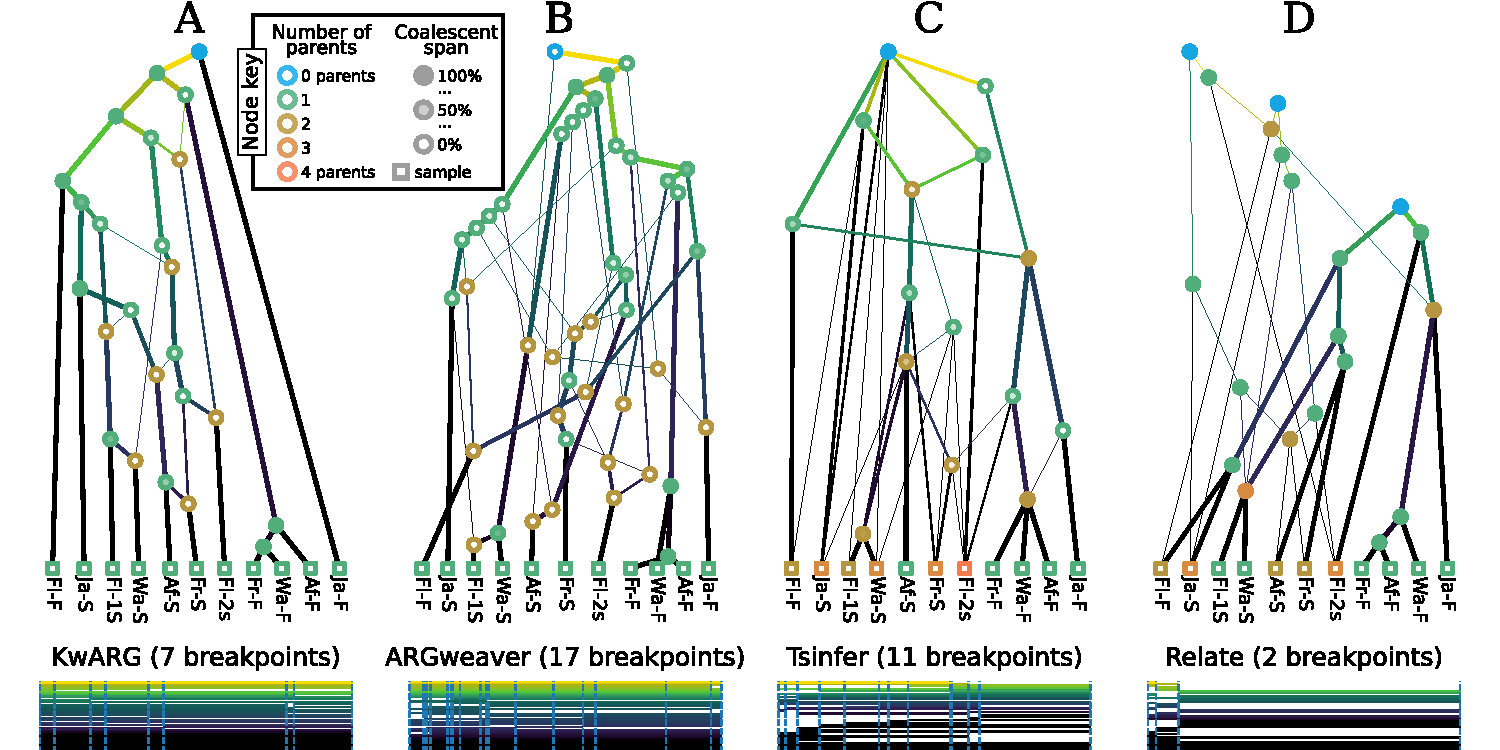
\includegraphics[width=\textwidth]{illustrations/inference.pdf}
\end{center}
\caption{\label{fig-inferred-args}
ARGs inferred by different methods from a 2.7kb region of the \textit{Drosophila melanogaster}
ADH locus for 11 samples~\citep{kreitman1983nucleotide}. Note that the position of points on the
Y axis is that chosen for graphical clarity by the graphviz \texttt{dot} algorithm,  rather than being
a direct measure of time. Additional notes about these ARGs.
}
\end{figure}

\section*{Discussion}

Discussion points (may or may not be used, certainly would be heavily revised)

\begin{itemize}
\item It is unfortunate that we are adding yet another meaning to the
term ARG here, but all we're really doing is making the implicit
assumptions that others have made (i.e., describing the output of
Relate, tsinfer etc as ARGs) and making them concrete. We need to have a
term to describe all of these things, and since people are already using
ARG for this, we might as well make it rigorous. We can then move away
from the unfruitful discussion about which methods infer a ``true'' or
``real'' ARG (none do, really, under the original definitions) and
instead start discussing the \emph{properties} of these ARGs. (See
next point also.)
\item Terminology based around an inferred ancestry being a ``true''
ARG is impoverished and misleading. The only reasonable interpretation
of a ARG being true or not is whether it's a sample from the coalescent.
Most inference methods (and all that scale well) do not. In any case,
the coalescent is just one model, and a highly idealised one. It is
exceedingly unlikely that the actual ARG describing the ancestry
of any biological population is ``true'' ARG in this sense. The terminology is
impoverished because it reduces the possibilities available
to something either being an ARG or not, whereas there are many different
interesting properties of these structures that we should be able to
discuss and compare.
\item tskit can represent any ARG.
\item Interchange is a real problem, and if we're going to realise the
potential for ARGs in genomics we must solve it. Efforts to standardise
phylogenetic networks haven't done very well (~\citep{cardona2008extended}
has 89 citations). The only real effort to standardise an ARG format
based on extending GraphML~\citep{mcgill2013graphml} has 11 citations.
GraphML~\citep{mcgill2013graphml} has some of the same key ideas
as tskit though, in particular allowing the annotation of ``live sites''
to an edge as a set of disjoint intervals that hold ancestral material.

\item There are real computational disadvantages to the Griffiths ARG
data structure. Having two types of node (three really, as we need
``sample'' nodes which are also treated differently) complicates algorithms,
and makes it difficult to reason about the structure of the ARG as a
graph. For example, there's some weirdness about mutations over
recombination nodes discussed by Gusfield [Ana?]

\item Comparison metrics are a problem. All evaluations has essentially
looked at either some form of pairwise comparison of trees along the genome
using tree metrics, or looked at the distributions of TMRCAs. No
one has succeeded in performing any comparisons of ARGs beyond
regarding them as a sequence of independent trees. If we genuinely believe
that ARGs are more than this, then we need to devise some metrics that
consider more than the local tree structure.

\item We should discuss other types of ancestry network also.
The crucial distiction between an ARG and a phylogenetic network (I think?) is
the presence of position information specifying the location of
recombination events (and by extension, the complete passage
of ancestral material the graph). Without position information
we know that a particular node was an ancestor somewhere along the
sequence, but not exactly where.

\item We make the point about expressivity of the eARG pretty
hard, but we don't mention anything about indels and structural
rearrangements etc. It's probably worth mentioning genome graphs
somewhere just to fend off this criticism. The high-level point
would be that it's unlikely to be easier to model this stuff
using node annotations.

\end{itemize}

% TODO not clear this belongs in the discussion, but we'll definitely
% want to make some of these points, even if they are being repeated
% from earlier section.
It is difficult to imagine a practical calculation performed on an
ARG that does not involve either the sequential generation of trees
along the genome or the resolved ancestry segments.
Knowing the resolved segments in an ancestry resolved gARG allows
us to perform many calculations without explicitly generating
the trees, and lets us work with the ancestry on a genome-by-genome
basis. We give three examples here. Firstly, generating mutations
on edges can be performed very quickly on an ancestry resolved
gARG, since we only need to examine $O(|E|)$ edges rather than
$O(nt)$ tree branches (assuming $n$ samples and $t$ marginal trees)
~\citep{baumdicker2021efficient}. If the ancestry were not resolved,
we would generate a large number of mutations on areas of the edge that
are non-ancestral. Secondly, computing the likelihood of a given
ARG realisation under the coalescent with recombination model
requires that we essentially recapitulate the state of Hudson's
algorithm (see XXX section) at each node in
the graph~\citep{baumdicker2021efficient}. Having resolved ancestry
substantially simplifies this process. Thirdly, computing
[FIXME describe what we did in tsdate]~\citep{wohns2022unified}.

Sequentially generating the marginal trees along the genome
is also fundamental, and is necessary whenever we need to
perform calculations that are contingent on more than just the
isolated properties of an edge. \cite{kelleher2016efficient}
showed how all trees can be sequentially generated in
constant time per tree transition in a fully simplified gARG.
Furthermore, we can easily reason about how tree topologies
change (and stay the same), leading to efficient algorithms
for computing population genetic
statistics~\citep{kelleher2016efficient,kelleher2018efficient},
implementing the Li and Stephens
model~\citep{kelleher2019inferring,wohns2022unified}
and likely many more.



\bibliographystyle{plainnat}
\bibliography{paper}

\end{document}
